%!TEX root = main.tex

\section{Definitions and key notation}\label{sec:dfin}

We use three notations for working with probability theory. The ``elementary'' notation makes use of regular symbolic conventions (functions, products, sums, integrals, unions etc.) along with the expectation operator $\mathbb{E}$. This is the most flexible notation which comes at the cost of being verbose and difficult to read. Secondly, we use a semi-formal string diagram notation extending the formal diagram notation for symmetric monoidal categories \cite{selinger_survey_2010}. Objects in this diagram refer to stochastic maps, and by interpreting diagrams as symbols we can, in theory, be just as flexible as the purely symbolic approach. However, we avoid complex mixtures of symbols and diagrams elements, and fall back to symbolic representations if it is called for. Finally, we use a matrix-vector product convention that isn't particularly expressive but can compactly express some common operations.

\subsection{Standard Symbols}

\begin{center}
\begin{tabular}{ |c|c|c| } 
 \hline
 Symbol & Meaning \\ 
 $[n]$& The natural numbers $\{1,...,n\}$ \\ 
 $f:a\mapsto b$ & Function definition, equivalent to $f(a):=b$\\
 Dots appearing in function arguments: $f(\cdot,\cdot,z)$ & The ``curried'' function $(x, y )\mapsto f(x,y,z)$\\
 Capital letters: $A,B, X$ & sets \\ 
 Script letters: $\mathcal{A},\mathcal{B},\mathcal{X}$ & $\sigma$-algebras on the sets $A, B, X$ respectively\\
 Script $\mathcal{G}$ & A directed acyclic graph made up of nodes $V$ and edges $E$\\
 Greek letters $\mu, \xi, \gamma$ & Probability measures\\
 $\delta_x$ & The Dirac delta measure: $\delta_x(A) = 1$ if $x\in A$ and $0$ otherwise\\
 Capital delta: $\Delta(\mathcal{E})$ & The set of all probability measures on $\mathcal{E}$\\
 Bold capitals: $\mathbf{A}$ & Markov kernel $\mathbf{A}:X\times\mathcal{Y}\to [0,1]$ (stochastic maps)\\
 Subscripted bold capitals: $\mathbf{A}_x$ & The probability measure given by the curried Markov kernel $\mathbf{A}(x,\cdot)$\\
 $A\to\Delta(\mathcal{B})$ & Markov kernel signature, treated as equivalent to $A\times \mathcal{B}\to [0,1]$\\
 $\mathbf{A}:x\mapsto \nu$ & Markov kernel definition, equivalent to $\mathbf{A}(x,B) = \nu(B)$ for all $B$\\
 Sans serif capitals: $\RV{A},\RV{X}$ & Measurable functions; we will also call them random variables\\
 $\mathbf{F}_{\RV{X}}$ & The Markov kernel associated with the function $\RV{X}$: $\mathbf{F}_{\RV{X}} \equiv a\mapsto \delta_{\RV{X}(a)}$\\
 $\mathbf{N}_{\RV{A}|\RV{B}}$ & The conditional probability (disintegration) of $\RV{A}$ given $\RV{B}$ under $\nu$\\
 $\nu \mathbf{F}_{\RV{X}}$ & The marginal distribution of $\RV{X}$ under $\nu$\\
 \hline
\end{tabular}
\end{center}

\subsection{Probability Theory}

Given a set $A$, a $\sigma$-algebra $\mathcal{A}$ is a collection of subsets of $A$ where
\begin{itemize}
	\item $A\in \mathcal{A}$ and $\emptyset\in \mathcal{A}$
	\item $B\in \mathcal{A}\implies B^C\in\mathcal{A}$
	\item $\mathcal{A}$ is closed under countable unions: For any countable collection $\{B_i|i\in Z\subset \mathbb{N}\}$ of elements of $\mathcal{A}$, $\cup_{i\in Z}B_i\in \mathcal{A}$ 
\end{itemize}

A measurable space $(A,\mathcal{A})$ is a set $A$ along with a $\sigma$-algebra $\mathcal{A}$. Sometimes the sigma algebra will be left implicit, in which case $A$ will just be introduced as a measurable space.

\paragraph{Common $\sigma$ algebras}

For any $A$, $\{\emptyset,A\}$ is a $\sigma$-algebra. In particular, it is the only sigma algebra for any one element set $\{*\}$.

For countable $A$, the power set $\mathscr{P}(A)$ is known as the discrete $\sigma$-algebra.

Given $A$ and a collection of subsets of $B\subset\mathscr{P}(A)$, $\sigma(B)$ is the smallest $\sigma$-algebra containing all the elements of $B$. 

Let $T$ be all the open subsets of $\mathbb{R}$. Then $\mathcal{B}(\mathbb{R}):=\sigma(T)$ is the \emph{Borel $\sigma$-algebra} on the reals. This definition extends to an arbitrary topological space $A$ with topology $T$.

A \emph{standard measurable set} is a measurable set $A$ that is isomorphic either to a discrete measurable space $A$ or $(\mathbb{R}, \mathcal{B}(\mathbb{R}))$. For any $A$ that is a complete separable metric space, $(A,\mathcal{B}(A))$ is standard measurable. 

Given a measurable space $(E,\mathcal{E})$, a map $\mu:\mathcal{E}\to [0,1]$ is a \emph{probability measure} if
\begin{itemize}
	\item $\mu(E)=1$, $\mu(\emptyset)=0$
	\item Given countable collection $\{A_i\}\subset\mathscr{E}$, $\mu(\cup_{i} A_i) = \sum_i \mu(A_i)$
\end{itemize}

Write by $\Delta(\mathcal{E})$ the set of all probability measures on $\mathcal{E}$.

Given a second measurable space $(F,\mathcal{F})$, a \emph{stochastic map} or \emph{Markov kernel} is a map $\mathbf{M}:E\times\mathcal{F}\to [0,1]$ such that
\begin{itemize}
	\item The map $\mathbf{M}(\cdot;A):x\mapsto \mathbf{M}(x;A)$ is $\mathcal{E}$-measurable for all $A\in \mathcal{F}$
	\item The map $\mathbf{M}_x:A\mapsto \mathbf{M}(x;A)$ is a probability measure on $F$ for all $x\in E$
\end{itemize}

Extending the subscript notation above, for $\mathbf{C}:X\times Y\to \Delta(\mathcal{Z})$  and $x\in X$ we will write $\mathbf{C}_x$ for the ``curried'' map $y\mapsto \mathbf{C}_{x,y}$.

The map $x\mapsto \mathbf{M}_x$ is of type $E\to \Delta(\mathcal{F})$. We will abuse notation somewhat to write $\mathbf{M}:E\to \Delta(\mathcal{F})$, which captures the intuition that a Markov kernel maps from elements of $E$ to probability measures on $\mathcal{F}$. Note that we ``reverse'' this idea and consider Markov kernels to map from elements of $\mathcal{F}$ to measurable functions $E\to[0,1]$, an interpretation found in \citet{clerc_pointless_2017}, but (at this stage) we don't make use of this interpretation here.

Given an indiscrete measurable space $(\{*\},\{\{*\},\emptyset\})$, we identify Markov kernels $\mathbf{N}:\{*\}\to \Delta(\mathcal{E})$ with the probability measure $\mathbf{N}_*$. In addition, there is a unique Markov kernel $\stopper{0.2}:E\to \Delta(\{\{*\},\emptyset\})$ given by $x\mapsto \delta_*$ for all $x\in E$ which we will call the ``discard'' map.


\subsection{Product Notation}

We can use a notation similar to the standard notation for matrix-vector products to represent operations with Markov kernels. Probability measures $\mu\in \Delta(\mathcal{X})$ can be read as row vectors, Markov kernels as matrices and measurable functions $\RV{T}:Y\to T$ as column vectors. Defining $\mathbf{M}:X\to \Delta(\mathcal{Y})$ and $\mathbf{N}:Y\to \Delta(\mathcal{Z})$, the measure-kernel product $\mu \mathbf{A} (G) := \int \mathbf{A}_x (G) d\mu(x)$ yields a probability measure $\mu\mathbf{A}$ on $\mathcal{Z}$, the kernel-kernel product $\mathbf{M}\mathbf{N}(x;H)=\int_Y \mathbf{B}(y;H)d\mathbf{A}_x$ yields a kernel $\mathbf{M}\mathbf{N}:X\to \Delta(\mathcal{Z})$ and the kernel-function product $\mathbf{A}\RV{T}(x):=\int_Y \RV{T}(y) d\mathbf{A}_x$ yields a measurable function $X\to T$. Kernel products are associative \citep{cinlar_probability_2011}.

The tensor product $(\mathbf{M}\otimes \mathbf{N})(x,y;G,H) := \mathbf{M}(x;G)\mathbf{N}(y;H)$ yields a kernel $(\mathbf{M}\otimes \mathbf{N}):X\times Y\to \Delta(\mathcal{Y}\otimes\mathcal{Z})$.

\subsection{String Diagrams}

Some constructions are unwieldly in product notation; for example, given $\mu\in \Delta(\mathcal{E})$ and $\mathbf{M}:E\to (\mathcal{F})$, it is not straightforward to construct a measure $\nu\in\Delta(\mathcal{E}\otimes\mathcal{F})$ that captures the ``joint distribution'' given by $A\times B\mapsto \int_A \mathbf{M}(x;B)d\mu$. 

Such constructions can, however, be straightforwardly captured with string diagrams, a notation developed for category theoretic probability. \citet{cho_disintegration_2019} also provides an extensive introduction to the notation discussed here.

Some key ideas of string diagrams:
\begin{itemize}
	\item Basic string diagrams can always be interpreted as a mixture of kernel-kernel products and tensor products of Markov kernels
	\begin{itemize}
	\item Extended string diagrams can be interepreted as a mixture of kernel-kernel products, kernel-function products, tensor products of kernels and functions and scalar products 
	\end{itemize}
	\item String diagrams are the subject of a coherence theorem: taking a string diagram and applying a planar deformation yields a string diagram that represents the same kernel \citep{selinger_survey_2010}. This also holds for a number of additional transformations detailed below
\end{itemize}

A kernel $\mathbf{M}:X\to \Delta(\mathcal{Y})$ is written as a box with input and output wires, probability measures $\mu\in \Delta(\mathcal{X})$ are written as triangles ``closed on the left'' and measurable functions (which are only elements of the ``extended'' notation) $\RV{T}:Y\to T$ as triangles ``closed on the right''. For this introduction we will label wires with the names of their corresponding spaces, but in practice we will usually name them with corresponding \emph{random variables}, though additional care is required when using random variables as labels (see paragraph \ref{par:random_variables}).

For $\mathbf{M}:X\to \Delta(\mathcal{Y})$, $\mu\in \Delta(\mathcal{X})$ and $f:X\to W$:

\begin{align}
\begin{tikzpicture}
\path (0,0) node (A) {$X$}
++(0.75,0) node[kernel] (B) {$\mathbf{M}$}
++(0.75,0) node (C) {$Y$};
\draw (A) -- (B) -- (C);
\end{tikzpicture}\qquad
\begin{tikzpicture}
\path (0,0) node[dist] (B) {$\mu$}
++(0.75,0) node (C) {$X$};
\draw (B) -- (C);
\end{tikzpicture}\qquad
\begin{tikzpicture}
\path (0,0) node (A) {$X$}
++(0.75,0) node[expectation] (B) {$f$};
\draw (A) -- (B);
\end{tikzpicture}
\end{align}

\paragraph{Basic and extended notation}

We canonically regard a probability measure $\mu\in \Delta(\mathcal{E})$ to be a Markov kernel $\mu:\{*\}\to \Delta(\mathcal{E})$. This allows for the definition of ``basic'' string diagrams for which Markov kernels are the only building blocks. Such a definition isn't possible for measurable functions. Suppose by analogy with the example probability measures and try to identify a measurable function $f:E\to \mathbb{R}$ with a Markov kernel $f':E\times\{*\}\to \mathbb{R}$. For $x\in E$ we cannot generally have both $f'(x,*)=1$ and $f'(x,*)=f(x)$, and so this attempt fails. This lack of normalisation is the reason we require an ``extended'' string diagram notation if we wish to incorporate functions and expectations which allows for the representation of scalars.


\paragraph{Elementary operations}

We can compose Markov kernels with appropriate spaces - the equivalent operation of the ``matrix products'' of product notation. Given $\mathbf{M}:X\to\Delta(\mathcal{Y})$ and $\mathbf{N}:Y\to \Delta(\mathcal{Z})$, we have 

\begin{align}
\mathbf{M}\mathbf{N} := \begin{tikzpicture}
 \path (0,0) node (E) {$X$}
 ++ (1,0) node[kernel] (M) {$\mathbf{M}$}
 ++ (1,0) node[kernel] (N) {$\mathbf{N}$}
 ++(1,0) node (G) {$Z$};
 \draw (E) -- (M) -- (N) -- (G);
\end{tikzpicture}\label{eq:sd_composition}
\end{align}

Probability measures are distinguished in that that they only admit ``right composition'' while functions only admit ``left composition''. For $\mu\in \Delta(\mathcal{E})$, $h:F\to X$:

\begin{align}
\mu\mathbf{M} &:= \begin{tikzpicture}
 \path (0,0) node[dist] (M) {$\mu$}
 ++ (1,0) node[kernel] (N) {$\mathbf{M}$}
 ++(1,0) node (G) {$Z$};
 \draw (M) -- (N) -- (G);
\end{tikzpicture}\\
\mathbf{M}f&:= \begin{tikzpicture}
 \path (0,0) node (E) {$X$}
 ++ (1,0) node[kernel] (M) {$\mathbf{M}$}
 ++ (1,0) node[expectation] (N) {$f$};
 \draw (E) -- (M) -- (N);
 \end{tikzpicture}
\end{align}


We can also combine Markov kernels using tensor products, which we represent with vertical juxtaposition. For $\mathbf{O}:Z\to \Delta(\mathcal{W})$:


\begin{align}
\mathbf{M}\otimes\mathbf{N}&:= \begin{tikzpicture}
\path (0,0) node (E) {$X$}
++(1,0) node[kernel] (M) {$\mathbf{M}$}
++(1,0) node (F) {$Y$}
(0,-0.5) node (F1) {$Z$}
++(1,0) node[kernel] (N) {$\mathbf{O}$}
+(1,0) node (G) {$W$};
\draw (E) -- (M) -- (F);
\draw (F1) -- (N) -- (G);
\end{tikzpicture}
\end{align}

Product spaces can be represented either by two parallel wires or a single wire:
\begin{align}
X\times Y \cong \mathrm{Id}_X\otimes \mathrm{Id}_Y &:= 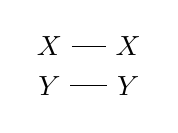
\begin{tikzpicture}
\path (0,0) node (E) {$X$}
++(1,0) node (F) {$X$}
(0,-0.5) node (F1) {$Y$}
+(1,0) node (G) {$Y$};
\draw (E) -- (F);
\draw (F1) -- (G);
\end{tikzpicture}\\
&= 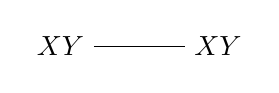
\begin{tikzpicture}
\path (0,0) node (X) {$X\utimes Y$}
++(2,0) node (Y) {$X\utimes Y$};
\draw (X) -- (Y);
\end{tikzpicture}
\end{align}

The notation $\RV{X}\utimes \RV{Y}$ will be explained in paragraph \ref{pgph:disint} - $\RV{X}\utimes\RV{Y}$ is a meta variable taking values in in the product space $X\times Y$.

Because a product space can be represented by parallel wires, a kernel $\mathbf{L}:X\to \Delta(\mathcal{Y}\otimes\mathcal{Z})$ can be written using either two parallel output wires or a single output wire:

\begin{align}
&\begin{tikzpicture}
\path (0,0) node (E) {$X$}
++ (1,0) node[kernel] (L) {$\mathbf{L}$}
++ (1,0.15) node (F) {$Y$}
+(0,-0.3) node (G) {$Z$};
\draw (E) -- (L);
\draw ($(L.east) + (0,0.15)$) -- (F);
\draw ($(L.east)+ (0,-0.15)$) -- (G);
\end{tikzpicture}\\
&\equiv\\
&\begin{tikzpicture}
\path (0,0) node (E) {$X$}
++ (1,0) node[kernel] (L) {$\mathbf{L}$}
++ (1.5,0) node (F) {$Y\utimes Z$};
\draw (E) -- (L) -- (F);
\end{tikzpicture}
\end{align}


\paragraph{Markov kernels with special notation}

A number of Markov kernels are given special notation distinct from the generic ``box'' representation above. These special representations facilitate intuitive graphical interpretations.

The identity kernel $\textbf{Id}:X\to \Delta(X)$ maps a point $x$ to the measure $\delta_x$ that places all mass on the same point:

\begin{align}
\textbf{Id}_x : x\mapsto \delta_x \equiv \begin{tikzpicture}\path (0,0) node (X) {$X$} + (1,0) node (X1) {$X$}; \draw (X)--(X1); \end{tikzpicture}\label{eq:identity}
\end{align}

The identity map preserves the name of a wire.

The copy map $\splitter{0.1}:X\to \Delta(\mathcal{X}\times \mathcal{X})$ maps a point $x$ to two identical copies of x:
\begin{align}
 \splitter{0.1}: x\mapsto \delta_{(x,x)} \equiv 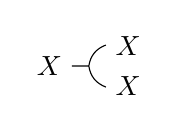
\begin{tikzpicture}
 \path (0,0) node (X) {$X$} ++ (0.5,0) coordinate (copy0) ++ (0.5,0.25) node (X1) {$X$} ++(0,-0.5) node (X2) {$X$};\draw (X)--(copy0) to [bend left] (X1) (copy0) to [bend right] (X2);
 \end{tikzpicture}\label{eq:copy}
 \end{align} 

Copy maps \emph{copy} the name of a wire. 

The swap map $\sigma:X\times Y\to \Delta(\mathcal{Y}\otimes\mathcal{X})$ swaps its inputs:

\begin{align}
\sigma := (x,y)\to \delta_{(y,x)} \equiv 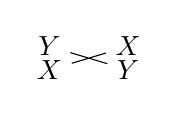
\begin{tikzpicture}
\path (0,0) node (X) {$X$}
+(1,0.3) node (X1) {$X$}
(0,0.3) node (Y) {$Y$}
+(1,-0.3) node (Y1) {$Y$};
\draw (X)--(X1) (Y) -- (Y1);
\end{tikzpicture}\label{eq:swap}
\end{align}

The swap map preserves the names of visually connected wires.

Apart from identity, copy and swap maps, we assign different names to the input and output wires of Markov kernels.

The discard map $\stopper{0.2}:X\to \Delta(\{*\})$ maps every input to $\delta_{*}$. Note that the only non-empty event in $\{\emptyset,\{*\}\}$ must have probability 1.
\begin{align}
\stopper{0.2}: x\mapsto \delta_{*} \equiv \begin{tikzpicture}
 \draw[-{Rays [n=8]}] (0,0) node (X) {$X$} (X) -- (1,0);
\end{tikzpicture}\label{eq:discard}
\end{align}

We can associate a Markov kernel $F\to \Delta(\mathcal{X})$ with any measurable function $F\to X$. A useful property of functional kernels is that products with functional kernels induce push-forward measures.

\begin{definition}[Function induced kernel]
Given a measurable function $g:F\to X$, define the function induced kernel $\mathbf{F}_{g}:F\to \Delta(\mathcal{X})$ to be the the Markov kernel $a\mapsto \delta_{g(a)}$ for all $a\in X$.
\end{definition}

\begin{definition}[Pushforward kernel]
Given a kernel $\mathbf{M}:E\to \Delta(\mathcal{F})$ and a measurable function $g:F\to X$, the \emph{pushforward kernel} $g_\# \mathbf{M}:E\to \Delta(\mathcal{X})$ is the kernel such that $g_\# \mathbf{M} (a;B) = \mathbf{M}(a;g^{-1}(B))$.

If $E$ is the indiscrete space $\{*\}$, then $\mathbf{M}$ can be identified with the probability measure $\mu:=\mathbf{M}_*$ and the pushforwark kernel $g_{\#}\mathbf{M}$ identified with the pushforward measure $g_{\#} \mu$, so pushforward kernels reduce to pushforward measures.
\end{definition}

\begin{lemma}[Pushforward kernels are functional kernel products]\label{lem:pushf_funk}
Given a kernel $\mathbf{M}:E\to \Delta(\mathcal{F})$ and a measurable function $g:F\to X$,the pushforward $g_\# \mathbf{M} = \mathbf{M} \mathbf{F}_{g}$.
\end{lemma}

\begin{proof}
\begin{align}
	\mathbf{M}\mathbf{F}_g(a;B) &= \int_F \delta_{g(y)}(B) d\mathbf{M}_a(y)\\
								&= \int_F \delta_{y}(g^{-1}(B)) d\mathbf{M}_a(y)\\
								&= \int_{g^{-1}(B)} d\mathbf{M}_a(y)\\
								&= g_{\#} \mathbf{M} (a;B)
\end{align}
\end{proof}


\subsubsection{Comparison of notations}

We are in a position to compare the three introduced notations using a few examples. Given $\mu\in\Delta(X),\mathbf{A}:X\to \Delta(Y)$ and $A\in \mathcal{X}$, $B\in\mathcal{Y}$, the following correspondences hold, where we express the same object in elementary notation, product notation and string notation respectively:

\begin{align}
\nu:=A\times B\mapsto \int_A A(x;B)d\mu(x) \equiv \mu \splitter{0.1}(\textbf{Id}_X\otimes \mathbf{A}) \equiv  \begin{tikzpicture}
\path (0,0) node[dist] (mu) {$\mu$}
++ (1,0) coordinate (copy0)
+ (1.2,0.5) node (X) {$X$}
++ (0.5,-0.5) node[kernel] (A) {$\mathbf{A}$}
++(0.7,0) node (Y) {$Y$};
\draw (mu)--(copy0);
\draw (copy0) to [bend left] (X);
\draw (copy0) to [bend right] (A) (A) -- (Y);
\end{tikzpicture}\label{eq:joint_measure}
\end{align}

Where the resulting object is a probability measure $\nu\in \Delta(\mathcal{X}\otimes\mathcal{Y})$. Note that the elementary notation requires a function definition here, while the product and string notations can represent the measure without explicitly addressing its action on various inputs and outputs. \citet{cho_disintegration_2019} calls this construction ``integrating $\mathbf{A}$ with respect to $\mu$''.

Define the marginal $\nu_Y\in \Delta(\mathcal{Y}):B\mapsto \nu(X\times B)$ for $B\in \mathcal{Y}$ and similarly for $\nu_X$. We can then express the result of marginalising \ref{eq:joint_measure} over $X$ in our three separate notations as follows:
\begin{align}
  \nu_Y (B) &= \nu(X\times B) = \int_X A(x;B) d\mu(x)\label{eq:marginalisation_elem}\\
  \nu_Y &= \mu \mathbf{A} = \mu \splitter{0.1}(\textbf{Id}_X\otimes \mathbf{A})(\stopper{0.2}\otimes \textbf{Id}_Y)\label{eq:marginalisation_prod}\\
  \nu_Y &= \begin{tikzpicture}
\path (0,0) node[dist] (mu) {$\mu$} ++ (1,0) node[kernel] (A) {$\mathbf{A}$} ++ (0.7,0) node (Y) {$Y$}; \draw (mu) -- (A) -- (Y);
\end{tikzpicture} = \begin{tikzpicture}
\path (0,0) node[dist] (mu) {$\mu$}
++ (1,0) coordinate (copy0)
+ (1.2,0.5) node (X) {}
++ (0.5,-0.5) node[kernel] (A) {$\mathbf{A}$}
++(0.7,0) node (Y) {$Y$};
\draw (mu)--(copy0);
\draw[-{Rays [n=8]}] (copy0) to [bend left] (X);
\draw (copy0) to [bend right] (A) (A) -- (Y);
\end{tikzpicture}\label{eq:marginalisation_graph}
\end{align}

The elementary notation \ref{eq:marginalisation_elem} makes the relationship between $\nu_Y$ and $\nu$ explicit and, again, requires the action on each event to be defined. The product notation \ref{eq:marginalisation_prod} is, in my view, the least transparent but also the most compact in the form $\mu \mathbf{A}$, and does not demand the explicit definition of how $\nu_Y$ treats every event. The graphical notation is the least compact in terms of space taken up on the page, but unlike the product notation it shows a clear relationship to the graphical construction in\ref{eq:joint_measure}, and displays a clear graphical logic whereby marginalisation corresponds to ``cutting off branches''. Like product notation, it also allows for the definition of derived measures such as $\nu_Y$ without explicit definition of the handling of all events. It also features a much smaller collection of symbols than does elementary notation.

String diagrams often achieve a good balance between interpretational transparency, expressive power and symbol economy. Downsides of string diagrams are that they can be time consuming to typeset, and formal reasoning with them takes some practice.


\subsubsection{Random Variables}\label{par:random_variables}

The summary of this section is:
\begin{itemize}
\item We label wires with the names of random variables
\item Diagrams with random variable labeled wires correspond to conditional/marginal distributions of those random variables in the obvious way
\item We work with \emph{conditional probability spaces} which are like probability spaces except some random variables don't have marginal distributions
\end{itemize}

Probability theory is primarily concerned with the behaviour of \emph{random variables}. This behaviour can be analysed via a collection of probability measures and Markov kernels representing joint, marginal and conditional distributions of random variables of interest. In the framework developed by Kolmogorov, this collection of joint, marginal and conditional distributions is modeled by a single underlying \emph{probability space}, and random variables by measurable functions on the probability space. 

We use the same approach here, with a couple of additions. 

\begin{enumerate}
	\item First, we are interested in variables whose outcomes depend both on random processes and decisions. These variables are better modelled by a Markov kernels than probability measure - \emph{given} a particular decision, they inherit a particular probability distribution. Thus, variables in our work are modeled by an underlying Markov kernel rather than a probability measure; we call this a \emph{conditional probability space}
	\item Secondly, we show how Markov kernel diagrams representing joint, marginal and conditional distributions within a conditional probability space can be identified by labels on the wires, analogously to the argument labels in $\mathbb{P}(\RV{X},\RV{Y})$ identifying the joint distribution of $\RV{X}$ and $\RV{Y}$ 
\end{enumerate}

With regard to the first point, \citet{hajek_what_2003} notes that there are many Markov kernels that cannot be uniquely specified by conditionals of probability measures. Thus, in general, conditional probability spaces cannot be identified with probability spaces. However, rather than dealing with the issues raised by this possibility, we limit ourselves to conditional probability spaces that can be identified with probability spaces.

As a general motivation, suppose the following identity holding for some $\mu$, $\mathbf{K}$:

\begin{align}
\begin{tikzpicture}
\path (0,0) node[dist] (m) {$\mathbb{P}$}
++ (0.7,0.15) node (E) {}
++ (0,-0.3) node (F) {};
\draw ($(m.east) + (0,0.15)$) -- (E);
\draw ($(m.east) + (0,-0.15)$) -- (F);
\end{tikzpicture} = \begin{tikzpicture}
\path (0,0) node[dist] (m) {$\mathbb{P}$}
++ (0.7,0.15) coordinate (copy0)
+(0,-0.3) node (Fs) {}
++ (1.2,0) node (E) {}
++(-0.7,-0.3) node[kernel] (K) {$\mathbf{K}$}
++(0.7,0) node (F) {};
\draw ($(m.east) + (0,0.15)$) -- (E);
\draw (copy0) to [bend right] (K) (K) -- (F);
\draw[-{Rays [n=8]}] ($(m.east) + (0,-0.15)$) -- (Fs);
\end{tikzpicture}\label{eq:disint_example}
\end{align}

This implies, roughly, that $\mathbf{K}$ is the probability of the lower wire of $\mu$ conditional on the upper (it is a \emph{disintegration} of $\mu$, defined later). We will want to deal with conditional probabilities such as $\mathbf{K}$ regularly; presently, we need to explicitly introduce $\mathbf{K}$ in a diagram such as \ref{eq:disint_example} to define it as such. Doing this every time we want a conditional probability makes the text much longer, and introduces mental overhead to the reader. Instead, we will adopt a system whereby the wires of a distinguished probability measure (or general Markov kernel) have names:

\begin{align}
\begin{tikzpicture}
\path (0,0) node[dist] (m) {$\mathbb{P}$}
++ (0.7,0.15) node (E) {$\RV{X}$}
++ (0,-0.3) node (F) {$\RV{Y}$};
\draw ($(m.east) + (0,0.15)$) -- (E);
\draw ($(m.east) + (0,-0.15)$) -- (F);
\end{tikzpicture}
\end{align}

And then we adopt the convention that any kernel labelled as

\begin{align}
\begin{tikzpicture}
\path (0,0) node (X) {$\RV{X}$}
++ (0.75,0) node[kernel] (E) {$\mathbb{P}_{\RV{Y}|\RV{X}}$}
++ (0.75,0) node (F) {$\RV{Y}$};
\draw (X) -- (E);
\draw (E) -- (F);
\end{tikzpicture}
\end{align}

satisfies Equation \ref{eq:disint_example} when substituted for $\mathbf{K}$.




\begin{definition}[Probability space, conditional probability space]
A \emph{probability space} $(\mathbb{P},\Omega,\mathcal{F})$ is a probability measure $\mathbb{P}$, which we call the \emph{ambient measure}, along with the \emph{sample space} $\Omega$ and the \emph{events} $\mathcal{F}$.

A \emph{conditional probability space} $(\mathscr{K},\Omega,\mathcal{F},D,\mathcal{D})$ is a Markov kernel $\mathscr{K}$, called the \emph{ambient kernel}, along with the sample space $\Omega$ and the \emph{input space} $D$.
\end{definition}

Note that we use the blackboard and script fonts to distinguish ambient measures and kernels. They are formally the same thing as ordinary probability measures and kernels, but it is useful to distinguish them to clarify the conventions we introduce in this section.

\begin{definition}[Random variable]
Given a sample space $\Omega$ and an input space $D$, a random variable $\RV{X}$ is a measurable function $\Omega\times D\to E$ for arbitrary measurable $E$. If the input space is trivial, it is simply a measurable function $\Omega\to X$.

We call the random variable $\RV{D}:\Omega\times D\to D$ given by $(w,d)\mapsto d$ to be the \emph{global conditioning variable}. $\RV{D}$ does not have a marginal distribution on a nontrivial conditional probability space (i.e. we don't have $D$ isomorphic to the indiscrete set $\{*\}$).
\end{definition}

\begin{definition}[Coupled tensor product $\utimes$]
Given two Markov kernels $\mathbf{M}$ and $\mathbf{N}$ or functions $f$ and $g$ with shared domain $E$, let $\mathbf{M}\utimes\mathbf{N}:=\splitter{0.1}(\mathbf{M}\otimes\mathbf{N})$ and $f\utimes g:=\splitter{0.1}(f\otimes g)$ where these expressions are interpreted using standard product notation. Graphically:

\begin{align}
\mathbf{M}\utimes\mathbf{N}&:=\begin{tikzpicture}
\path (0,0) node (E) {$E$}
++(0.5,0) coordinate (copy0)
+ (0.5,0.3) node[kernel] (M) {$\mathbf{M}$}
+(1.2,0.3) node (X) {$\RV{X}$}
+ (0.5,-0.3) node[kernel] (N) {$\mathbf{N}$}
+(1.2,-0.3) node (Y) {$\RV{Y}$};
\draw (E) -- (copy0) to [bend left] (M) (copy0) to [bend right] (N);
\draw (M) -- (X) (N) -- (Y);
\end{tikzpicture}\\
f\utimes g&:= \begin{tikzpicture}[scale=1.2]\path (0,0) node (E) {$E$}
++(0.5,0) coordinate (copy0)
+ (0.5,0.3) node[expectation] (M) {$f$}
+ (0.5,-0.3) node[expectation] (N) {$g$};
\draw (E) -- (copy0) to [bend left] (M) (copy0) to [bend right] (N);
\end{tikzpicture}
\end{align}
The operation denoted by $\utimes$ is associative (Lemma \ref{lem:utimes_assoc}), so we can without ambiguity write $f\utimes g\utimes ...\utimes h$ for finite groups of functions or Markov kernels sharing a domain. 
\end{definition}

\begin{lemma}[$\utimes$ is associative]\label{lem:utimes_assoc}
For Markov kernels $\mathbf{L}$, $\mathbf{M}$ and $\mathbf{N}$ sharing a domain $E$, $(\mathbf{L}\utimes\mathbf{M})\utimes\mathbf{N}=\mathbf{L}\utimes(\mathbf{M}\utimes\mathbf{N})$.
\end{lemma}

\begin{definition}[Marginal distribution, marginal kernel]\label{def:marginal_distribution}
Given $\mathbb{P}\in \Delta(\mathcal{F})$, random variable $\RV{X}:\Omega\to G$ the \emph{marginal distribution} of $\RV{X}$ $\mathbb{P}_{\RV{X}}\in \Delta(\mathcal{G})$ of $\RV{X}$ is the product measure $\mathbb{P}\mathbf{F}_{\RV{X}}$.

See Lemma \ref{lem:pushf_funk} for the proof that this matches the usual definition of marginal distribution.

Following this, given $\mathscr{K}:D\to \Delta(\mathcal{F})$ and random variable $\RV{X}:\Omega\to G$, the \emph{marginal kernel} is $\mathscr{K}\mathbf{F}_{\RV{X}}$.
\end{definition}

\begin{definition}[Joint distribution, joint kernel]\label{def:joint_distribution}
Given $\mathbb{P}\in \Delta(\mathcal{F})$, $\RV{X}:\Omega\to G$ and $\RV{Y}:\Omega\to H$, the \emph{joint distribution} $\mathbb{P}_{\RV{X}\RV{Y}}\in \Delta(\mathcal{G}\otimes\mathcal{H})$ of $\RV{X}$ and $\RV{Y}$ is the marginal distribution of $\RV{X}\utimes\RV{Y}$.

This is identical to the definition in, for example, \citet{cinlar_probability_2011} if we note that the random variable $(\RV{X},\RV{Y}):\omega\mapsto (\RV{X}(\omega),\RV{Y}(\omega))$ (\c{C}inlar's definition) is the same thing as $\RV{X}\utimes\RV{Y}$.

Analogously, the joint kernel $\mathscr{K}_{\RV{Y}|\RV{X}}$ is the product $\mathscr{K}\mathbb{F}_{\RV{X}\utimes\RV{Y}}$.
\end{definition}

Joint distributions have a nice visual representation, as a result of Lemma \ref{lem:jdist_cprod} which follows.

\begin{lemma}[Joint distributions and coupled products]\label{lem:jdist_cprod}
Given $\RV{X}:\Omega\to G$ and $\RV{Y}:\Omega\to H$, $\mathbf{F}_{\RV{X}\utimes\RV{Y}}=\mathbf{F}_\RV{X}\utimes\mathbf{F}_\RV{Y}$
\end{lemma}

\begin{proof}
For $a\in \Omega$, $B\in \mathcal{G}$, $C\in \mathcal{H}$,
\begin{align}
\mathbf{F}_{\RV{X}\utimes\RV{Y}} (a;B\times C) &= \delta_{\RV{X}(a),\RV{Y}(a)}(B\times C)\\
									   &= \delta_{\RV{X}(a)}(B)\delta_{\RV{Y}(a)}(C)\\
									   &= (\delta_{\RV{X}(a)}\otimes\delta_{\RV{Y}(a)})(B\times C)\\
									   &= \mathbf{F}_{\RV{X}}\utimes\mathbf{F}_{\RV{Y}}
\end{align}
Equality follows from the monotone class theorem.
\end{proof}

Therefore the following holds:

\begin{align}
\begin{tikzpicture}
\path (0,0) node (O) {}
++(0.7,0) node[kernel] (K) {$\mathscr{K}_{\RV{X}\RV{Y}}$}
++ (0.7,0.15) node (X) {}
+(0,-0.3) node (Y) {};
\draw (O) -- (K);
\draw ($(K.east) + (0,0.15)$) -- (X);
\draw ($(K.east) + (0,-0.15)$) -- (Y);
\end{tikzpicture}=
\begin{tikzpicture}
\path (0,0) node (O) {}
++ (0.7, 0) node[kernel] (K) {$\mathscr{K}$}
++ (0.6,0) coordinate (copy0)
++ (0.4,0.25) node[kernel] (X) {$\mathbf{F}_{\RV{X}}$}
+(0,-0.5) node[kernel] (Y) {$\mathbf{F}_{\RV{Y}}$}
++(0.6,0) node (Xo) {}
+(0,-0.5) node (Yo) {};
\draw (O) -- (K) -- (copy0);
\draw (copy0) to [bend left] (X) (X) -- (Xo);
\draw (copy0) to [bend right] (Y) (Y) -- (Yo);
\end{tikzpicture}
\end{align}


We are now in a position to define wire labels for ``output'' wires.

\begin{definition}[Wire labels - joint probabilities]\label{def:wl_jprob}
Given a conditional probability space with ambient kernel $\mathscr{K}:D\to \Delta(\mathcal{F})$ (or a probability space with measure $\mathbb{P}$) and some collection of random variables $\RV{X}$, $\RV{Y}$, ... on $\Omega\times D$, any diagram representing a kernel $\mathbf{L}:D\to \Delta(\mathcal{E})$ with \emph{output} wires labeled $\RV{X}$, $\RV{Y}$,...  represents the corresponding marginal of $\mathscr{K}$ (we assume that the space $E$ factorises appropriately). For example
\begin{align}
\begin{tikzpicture}
\path (0,0) node (A) {}
++ (0.7,0) node[kernel] (m) {$\mathbf{L}$}
++ (0.7,0.15) node (E) {$\RV{X}$}
++ (0,-0.3) node (F) {$\RV{Y}$};
\draw (A) -- (m) ($(m.east) + (0,0.15)$) -- (E);
\draw ($(m.east) + (0,-0.15)$) -- (F);
\end{tikzpicture}
\end{align}

asserts that $\mathbf{L}= \mathbf{K}_{\RV{X}\RV{Y}}$, the joint kernel of $\RV{X}$ and $\RV{Y}$.

If we have an ambient measure $\mathbb{P}$, then $D=\{*\}$ and the diagram
\begin{align}
\begin{tikzpicture}
\path (0,0) node[dist] (m) {$\mu$}
++ (0.7,0.15) node (E) {$\RV{X}$}
++ (0,-0.3) node (F) {$\RV{Y}$};
\draw ($(m.east) + (0,0.15)$) -- (E);
\draw ($(m.east) + (0,-0.15)$) -- (F);
\end{tikzpicture}
\end{align}

asserts that $\mu = \mathbb{P}_{\RV{X}\RV{Y}}$.

\end{definition}


\begin{definition}[Disintegration]\label{def:disintegration}
Given a probability space $(\mathbb{P},\Omega,\mathcal{F})$, random variables $\RV{X}$ and $\RV{Y}$ and joint probability measure $\mu:=\mathbb{P}_{\RV{X}\RV{Y}}\in \Delta(\mathcal{E}\otimes\mathcal{F})$, we say that $\mathbf{M}:E\to \Delta(\mathcal{F})$ is a disintegration of $\mu$ if
\begin{align}
\begin{tikzpicture}
\path (0,0) node[dist] (m) {$\mu$}
++ (0.7,0.15) node (E) {$\RV{X}$}
++ (0,-0.3) node (F) {$\RV{Y}$};
\draw ($(m.east) + (0,0.15)$) -- (E);
\draw ($(m.east) + (0,-0.15)$) -- (F);
\end{tikzpicture} = \begin{tikzpicture}
\path (0,0) node[dist] (m) {$\mu$}
++ (0.7,0.15) coordinate (copy0)
+(0.2,-0.3) node (T) {}
++ (1.2,0) node (E) {$\RV{X}$}
++(-0.7,-0.3) node[kernel] (K) {$\mathbf{M}$}
++(0.7,0) node (F) {$\RV{Y}$};
\draw ($(m.east) + (0,0.15)$) -- (E);
\draw (copy0) to [bend right] (K) (K) -- (F);
\draw[-{Rays [n=8]}] ($(m.east) + (0,-0.15)$) -- (T);
\end{tikzpicture}
\end{align}
Notationally, $\mathbf{N}$ is a version of $\mathbb{P}_{\RV{Y}|\RV{X}}$, ``the probability of $\RV{Y}$ given $\RV{X}$'', or $\mathbf{M}\in \mathbb{P}_{\RV{Y}|\RV{X}}$.

Given a conditional probability space $(\mathscr{K},\Omega,D)$, define $\mathscr{K}^*$ to be the kernel
\begin{align}
\begin{tikzpicture}
\path (0,0) node (O) {}
++(0.5,0) coordinate (copy0)
++ (0.5,0) node[kernel] (m) {$\mathscr{K}$}
++ (0.7,0.15) node (E) {}
++ (0,-0.3) node (F) {}
++(0,-0.3) node (G) {};
\draw (O) -- (m) ($(m.east) + (0,0.15)$) -- (E);
\draw ($(m.east) + (0,-0.15)$) -- (F);
\draw (copy0) to [bend right] (G);
\end{tikzpicture}
\end{align}

Given random variables $\RV{X},\RV{Y}$ on $\Omega\times D$ and kernel $\mathbf{L}:=\mathscr{K}^*_{\RV{X},\RV{Y}}:D\to \Delta(\mathcal{E}\otimes\mathcal{F})$, we say that $\mathbf{M}:D\times E\to \Delta(\mathcal{F})$ is a disintegration of $\mathbf{L}$ if

\begin{align}
\begin{tikzpicture}
\path (0,0) node (O) {}
++ (0.7,0) node[kernel] (m) {$\mathbf{L}$}
++ (0.7,0.15) node (E) {$\RV{X}$}
++ (0,-0.3) node (F) {$\RV{Y}$};
\draw (O) -- (m) ($(m.east) + (0,0.15)$) -- (E);
\draw ($(m.east) + (0,-0.15)$) -- (F);
\end{tikzpicture} = \begin{tikzpicture}
\path (0,0) node (O) {}
++ (0.3,0) coordinate (copy1)
++ (0.5,0) node[kernel] (m) {$\mathbf{L}$}
++ (0.7,0.15) coordinate (copy0)
+(0.2,-0.3) node (T) {}
++ (1.2,0) node (E) {$\RV{X}$}
++(-0.7,-0.3) node[kernel] (K) {$\mathbf{M}$}
++(0.7,0) node (F) {$\RV{Y}$};
\draw (O) -- (m) ($(m.east) + (0,0.15)$) -- (E);
\draw (copy0) to [bend right] (K) (K) -- (F);
\draw (copy1) to [out=270,in=180] ($(K.west) + (0,-0.15)$);
\draw[-{Rays [n=8]}] ($(m.east) + (0,-0.15)$) -- (T);
\end{tikzpicture}\label{eq:def_k_disint}
\end{align}

Similarly, recalling that $\RV{D}$ is the global conditioning variable, we can say $\mathbf{M}\in \mathscr{K}_{\RV{Y}|\RV{X}\RV{D}}$. We require disintegrations of kernel spaces to be conditional on the global conditioning variable, as this along with certain other conditions guarantees the existence of a disintegration.

Note that Eq. \ref{eq:def_k_disint} also implies
\begin{align}
\begin{tikzpicture}
\path (0,0) node (O) {}
++(0.5,0) coordinate (copy1)
++ (0.7,0) node[kernel] (m) {$\mathbf{L}$}
++ (0.7,0.15) node (E) {$\RV{X}$}
++ (0,-0.3) node (F) {$\RV{Y}$}
++(0,-0.3) node (D) {$\RV{D}$};
\draw (O) -- (m) ($(m.east) + (0,0.15)$) -- (E);
\draw ($(m.east) + (0,-0.15)$) -- (F);
\draw (copy1) to [bend right] (D);
\end{tikzpicture} = \begin{tikzpicture}
\path (0,0) node (O) {}
++(0.3,0) coordinate (copy2)
++ (0.3,0) coordinate (copy1)
++ (0.5,0) node[kernel] (m) {$\mathbf{L}$}
++ (0.7,0.15) coordinate (copy0)
+(0.2,-0.3) node (T) {}
++ (1.2,0) node (E) {$\RV{X}$}
++(-0.7,-0.3) node[kernel] (K) {$\mathbf{M}$}
++(0.7,0) node (F) {$\RV{Y}$}
++(0,-0.4) node (D) {$\RV{D}$};
\draw (O) -- (m) ($(m.east) + (0,0.15)$) -- (E);
\draw (copy0) to [bend right] (K) (K) -- (F);
\draw (copy1) to [out=270,in=180] ($(K.west) + (0,-0.15)$);
\draw[-{Rays [n=8]}] ($(m.east) + (0,-0.15)$) -- (T);
\draw (copy2) to [bend right] (D);
\end{tikzpicture}\label{eq:def_k_disint}
\end{align}

\end{definition}

\begin{definition}[Wire labels - disintegrations]\label{def:wl_disint}
Given a conditional probability space with ambient kernel $\mathscr{K}:D\to \Delta(\mathcal{F})$ (or a probability space with measure $\mathbb{P}$), 

Note that $\mathbb{P}^*$ is simply $\mathbb{P}$ for a probability space

Recall that $\RV{D}$ is the global conditioning variable. Given two collections of random variables $c_1 = [\RV{X}_1,\RV{X}_2,...]$ and $c_2 = [\RV{Y}_1,\RV{Y}_2]$, we adopt the convention that any diagram with the input wires labeled with $c_1$ and the output wires labeled with $c_2$ is an element of $\mathscr{K}^*_{\RV{Y_1Y_2...}|\RV{X}_1\RV{X}_2...}$. 

That is, by this convention, the diagram

\begin{align}
\begin{tikzpicture}
\path (0,0) node (O) {$\RV{X}$}
++(0,-0.3) node (D) {$\RV{D}$}
++ (0.7,0.15) node[kernel] (m) {$\mathbf{M}$}
++ (0.7,0) node (E) {$\RV{Y}$};
\draw (O) -- ($(m.west)+(0,0.15)$) (m) -- (E);
\draw (D) -- ($(m.west)+(0,-0.15)$);
\end{tikzpicture}
\end{align}

implies that $\mathbf{M}\in\mathscr{K}_{\RV{Y}|\RV{X}\RV{D}}$. Note further that by Theorem \ref{th:disintegration_exist_ker}, we can rely on the existence of disintegrations such as $\mathbf{M}$ that are conditional on the global conditioning variable $\RV{D}$ provided we have countable $D$ and standard measurable $(Y,\mathcal{Y})$.

If we have some version $\mathbf{M}$ of $\mathscr{K}_{\RV{Y}|\RV{X}\RV{D}}$ that does not depend on the value of $\RV{D}$ - i.e. $\mathbf{M}_{(x,d)}=\mathbf{M}_{(x,d')}$ for all $x\in X$, $d,d'\in D$, then there exists some $\mathbf{M}'$ such that:

\begin{align}
\begin{tikzpicture}
\path (0,0) node (O) {$\RV{X}$}
++(0,-0.3) node (D) {$\RV{D}$}
++ (0.7,0.15) node[kernel] (m) {$\mathbf{M}$}
++ (0.7,0) node (E) {$\RV{Y}$};
\draw (O) -- ($(m.west)+(0,0.15)$) (m) -- (E);
\draw (D) -- ($(m.west)+(0,-0.15)$);
\end{tikzpicture} = 
\begin{tikzpicture}
\path (0,0) node (O) {$\RV{X}$}
+(0,-0.5) node (OD) {$\RV{D}$}
++ (0.7,0) node[kernel] (m) {$\mathbf{M}'$}
++ (0.7,0) node (E) {$\RV{Y}$}
+(0,-0.5) node (S) {};
\draw (O) -- (m) -- (E);
\draw[-{Rays [n=8]}] (OD) -- (S);
\end{tikzpicture}\label{eq:indep_of_D}
\end{align}

Under these circumstances, we will abuse notation to say $\mathbf{M}'=\mathscr{K}_{\RV{Y}|\RV{X}}$.

\end{definition}

We can't expect Equation \ref{eq:indep_of_D} to hold in an arbitrary conditional probability spaces. For a very simple example, take $\mathscr{K}:\{0,1\}\to \Delta(\{0,1\})$ where $\mathscr{K}_0=\mathscr{K}_1=\mathrm{Bernoulli}(0.5)$, and let $\RV{X}:(x,d)\mapsto x$ - i.e. the random variable projecting the output of $\mathscr{K}$. Then there is no disintegration $\mathscr{K}_{\RV{D}|\RV{X}}$ - we can't recover the input $\RV{D}$ from $\RV{X}$.

Under some (strong) regularity conditions, disintegrations of conditional probability spaces do exist.

\begin{theorem}[Disintegration existence - probability space]\label{th:disintegration_exist}
Given a probability measure $\mu\in \Delta(\mathcal{E}\otimes \mathcal{F})$, if $(F,\mathcal{F})$ is standard then a disintegration $\mathbf{K}:E\to \Delta(\mathcal{F})$ exists \citep{cinlar_probability_2011}.
\end{theorem}

\begin{theorem}[Disintegration existence - conditional probability space]\label{th:disintegration_exist_ker}
Given a kernel $\mathbf{L}:D\to \Delta(\mathcal{E}\otimes\mathcal{F})$, define $\mathbf{L}^*$:
\begin{align}
\begin{tikzpicture}
\path (0,0) node (O) {}
++(0.5,0) coordinate (copy0)
++ (0.5,0) node[kernel] (m) {$\mathbf{L}$}
++ (0.7,0.15) node (E) {}
++ (0,-0.3) node (F) {}
++(0,-0.3) node (G) {};
\draw (O) -- (m) ($(m.east) + (0,0.15)$) -- (E);
\draw ($(m.east) + (0,-0.15)$) -- (F);
\draw (copy0) to [bend right] (G);
\end{tikzpicture}
\end{align}

If $D$ is countable and $(F,\mathcal{F})$ is standard, then there is a disintegration $\mathbf{M}:D\times E\to \Delta(\mathcal{F})$ of $\mathbf{L}^*$.
\end{theorem}

\begin{proof}
By Theorem \ref{th:disintegration_exist}, for each $d\in D$ we have a disintegration $\mathbf{K}^{(d)}:E\to \Delta(\mathcal{F})$ of $\mathbf{L}_d$. Define $\mathbf{M}:D\times E\to \Delta(\mathcal{F})$ by $\mathbf{M} (d,e;A) = \mathbf{K}^{(d)} (e;A)$ for $d\in D$, $e\in E$, $A\in\mathcal{F}$. Clearly $\mathbf{M}_{(d,e)}$ is a probability measure. Furthermore, for $B\in \mathcal{B}(\mathbb{R})$, $\mathbf{M}^{-1}(\cdot;A)(B) = \cup_{d\in D} \{d\}\times \mathbf{K}^{(d)-1}(\cdot;A)(B)$, which is a countable union of measurable sets and therefore measurable. 
\end{proof}

In general, we don't want to spent time explicitly setting up conditional probability spaces. Rather, we will specify key marginals and disintegrations from which a conditional probability space can be constructed - call these marginals and conditional ``components''. Clearly we cannot build a conditional probability space from two kernels that represent the same component but disagree with each other on a non-negligible set. Also, in general, for an arbitrary collection of components there may be many ambient kernels from which we can extract these components. There is no particular problem if we have multiple ambient kernels over undefined random variable; if we are only interested in $\RV{X}$ then the possibility of many joint kernels over $\RV{X}$ and $\RV{Y}$ is no cause for concern. We do, however, want to avoid ambient kernels supporting non-negligibly distinct marginals or disintegrations over the random variables that have been defined. 

\begin{example}[Implicit conditional probability space]
Suppose we have labeled Markov kernels
\begin{align}
\begin{tikzpicture}
\path (0,0) node (X) {$\RV{D}$}
++ (0.7,0) node[kernel] (L) {$\mathbf{L}$}
++(0.7,0) node (Y) {$\RV{X}$};
\draw (X) -- (L) -- (Y);
\end{tikzpicture}\qquad
&\begin{tikzpicture}
\path (0,0) node (X) {$\RV{X}$}
++ (0.7,0) node[kernel] (L) {$\mathbf{M}$}
++(0.7,0) node (Y) {$\RV{Y}$};
\draw (X) -- (L) -- (Y);
\end{tikzpicture}
\end{align}
We want to define a conditional probability space $(\mathscr{K},\Omega,D)$ supporting random variables $\RV{D}$, $\RV{X}$ and $\RV{Y}$ yielding the above kernels as the relevant marginals and disintegrations. Strictly:
\begin{itemize}
	\item $\mathbf{L}=\mathscr{K}_{\RV{X}|\RV{D}}$
	\item $\mathbf{M}\otimes \stopper{0.3}_D \in \mathscr{K}_{\RV{Y}|\RV{X}{D}}$ (``informally'', $\mathbf{M}\in \mathscr{K}_{\RV{Y}|\RV{X}}$)
\end{itemize} 

Take $\Omega=W\times X\times Y\times Z$ and define $\mathscr{K}$ such that

\begin{align}
\mathscr{K}^* = \begin{tikzpicture}
\path (0,0) node (X) {$\RV{D}$}
++ (0.4,0) coordinate (copy1)
++ (0.5,0) node[kernel] (L) {$\mathbf{L}$}
++ (0.7,0) coordinate (copy2)
++ (0.7,0) node[kernel] (M) {$\mathbf{M}$}
++(0.7,0) node (Y) {$\RV{Y}$}
+(0,-0.4) node (X1) {$\RV{X}$}
+(0,-0.8) node (D) {$\RV{D}$};
\draw (X) -- (L) -- (M) -- (Y);
\draw (copy1) to [bend right] (D);
\draw (copy2) to [bend right] (X1);
\end{tikzpicture}
\end{align}

Where $\mathscr{K}^*$ is the copy map composed with $\mathscr{K}$ as in previous definitions. $\mathscr{K}$ is the unique Markov kernel $D\to \Delta(\mathcal{X}\otimes\mathcal{Y})$ supporting the two criteria above, assuming finite $D$ and standard measurable $X,Y$.

\begin{proof}
By assumption, for any suitable $\mathscr{K}':D\to \Delta(\mathcal{X}\otimes\mathcal{Y})$ we have

\begin{align}
\begin{tikzpicture}
\path (0,0) node (D) {$\RV{D}$}
++ (0.7,0) node[kernel] (K) {$\mathscr{K}'$}
++ (0.7,0.15) node (X) {$\RV{X}$}
+(0,-0.3) node (Y) {};
\draw (D) -- (K) ($(K.east) + (0,0.15)$) -- (X);
\draw[-{Rays [n=8]}] ($(K.east)+(0,-0.15)$) -- (Y);
\end{tikzpicture} &=
\begin{tikzpicture}
\path (0,0) node (X) {$\RV{D}$}
++ (0.7,0) node[kernel] (L) {$\mathbf{L}$}
++(0.7,0) node (Y) {$\RV{X}$};
\draw (X) -- (L) -- (Y);
\end{tikzpicture}
\end{align}

and by the fact that $\mathbf{M}\otimes \stopper{0.3}_D$ is by assumption a disintegration of $\mathscr{K}^{\prime*}$:

\begin{align}
\begin{tikzpicture}
\path (0,0) node (D) {$\RV{D}$}
++ (0.3,0) coordinate (copy0)
++ (0.5,0) node[kernel] (K) {$\mathscr{K}'$}
++ (0.7,0.15) node (X) {$\RV{X}$}
+(0,-0.3) node (Y) {$\RV{Y}$}
+(0,-0.6) node (D1) {$\RV{D}$};
\draw (D) -- (K) ($(K.east) + (0,0.15)$) -- (X);
\draw ($(K.east)+(0,-0.15)$) -- (Y);
\draw (copy0) to [bend right] (D1);
\end{tikzpicture}
&= 
\begin{tikzpicture}
\path (0,0) node (X) {$\RV{D}$}
++ (0.4,0) coordinate (copy1)
++ (0.5,0) node[kernel] (L) {$\mathscr{K}'$}
++ (0.7,0.15) coordinate (copy2)
+ (0,-0.3) node (Ys) {}
++ (0.7,0) node[kernel] (M) {$\mathbf{M}$}
++(0.7,0) node (Y) {$\RV{Y}$}
+(0,-0.4) node (X1) {$\RV{X}$}
+(0,-0.8) node (D) {$\RV{D}$};
\draw (X) -- (L) ($(L.east)+(0,0.15)$) -- (M) -- (Y);
\draw[-{Rays [n=8]}] ($(L.east)+(0,-0.15)$) -- (Ys);
\draw (copy1) to [bend right] (D);
\draw (copy2) to [bend right] (X1);
\draw[-{Rays [n=8]}] (copy1) to [bend left] ($(M.east) + (-0.05,0.3)$);
\end{tikzpicture}\\
&= \begin{tikzpicture}
\path (0,0) node (X) {$\RV{D}$}
++ (0.4,0) coordinate (copy1)
++ (0.5,0) node[kernel] (L) {$\mathbf{L}$}
++ (0.7,0) coordinate (copy2)
++ (0.7,0) node[kernel] (M) {$\mathbf{M}$}
++(0.7,0) node (Y) {$\RV{Y}$}
+(0,-0.4) node (X1) {$\RV{X}$}
+(0,-0.8) node (D) {$\RV{D}$};
\draw (X) -- (L) -- (M) -- (Y);
\draw (copy1) to [bend right] (D);
\draw (copy2) to [bend right] (X1);
\end{tikzpicture}
\end{align}

Finally, if $\mathscr{K}^* = \mathscr{K}^{\prime*}$, then at least if $D$ is countable we must have $\mathscr{K}=\mathscr{K}'$ as they must agree on all points in $D$.
\end{proof}


This example was chosen to illustrate a peculiarity of our notation of conditional probability spaces. Consider a problem that appears similar: find an ambient measure $\mathbb{P}$ decomposing into the following marginal and conditionals:

\begin{align}
\begin{tikzpicture}
\path (0,0) node[dist] (mu) {$\mu$}
++(0.7,0) node (D) {$\RV{D}$};
\draw (mu) -- (D);
\end{tikzpicture}\qquad
\begin{tikzpicture}
\path (0,0) node (X) {$\RV{D}$}
++ (0.7,0) node[kernel] (L) {$\mathbf{L}$}
++(0.7,0) node (Y) {$\RV{X}$};
\draw (X) -- (L) -- (Y);
\end{tikzpicture}\qquad
&\begin{tikzpicture}
\path (0,0) node (X) {$\RV{X}$}
++ (0.7,0) node[kernel] (L) {$\mathbf{M}$}
++(0.7,0) node (Y) {$\RV{Y}$};
\draw (X) -- (L) -- (Y);
\end{tikzpicture}
\end{align}

Here there are many choices of $\mathbb{P}$ that satisfy our conditions arising from different choices of $\mathbb{P}_{\RV{Y}|\RV{X}\RV{D}}$. This is not possible in the conditional probability space because $\mathscr{K}_{\RV{Y}|\RV{X}}$ only exists if $\mathscr{K}_{\RV{Y}|\RV{X}\RV{D}}$ is independent of $\RV{D}$. That is, in a conditional probability space every disintegration is conditional on $\RV{D}$, but we may not explicitly write this if it does not actually depend on $\RV{D}$.
\end{example}

A sufficient condition for the construction of a unique ambient kernel from a collection of components $\{C_1,...C_n\}$ is if there is some ordering of components $\{{i_1},{i_2},...{i_n}\}$ such that the input labels of $C_{i_{k+1}}$ is the union of the inputs and outputs of $C_{i_1},...,C_{i_j}$. This can be shown by repeated application of Theorem \ref{th:disintegration_exist_ker}.


% \begin{definition}[Labeled disintegration]\label{def:labeled_disint}
% Given a probability measure $\mu$ with labels $\RV{X}$ and $\RV{Y}$, we say that $\mathbf{K}$ is a version of the conditional probability of $\RV{Y}$ given $\RV{X}$ if
% \begin{align}
% \begin{tikzpicture}
% \path (0,0) node[dist] (m) {$\mu$}
% ++ (0.7,0.15) node (E) {$\RV{X}$}
% ++ (0,-0.3) node (F) {$\RV{Y}$};
% \draw ($(m.east) + (0,0.15)$) -- (E);
% \draw ($(m.east) + (0,-0.15)$) -- (F);
% \end{tikzpicture} = \begin{tikzpicture}
% \path (0,0) node[dist] (m) {$\mu$}
% ++ (0.7,0.15) coordinate (copy0)
% ++ (1.2,0) node (E) {$\RV{X}$}
% ++(-0.7,-0.3) node[kernel] (K) {$\mathbf{K}$}
% ++(0.7,0) node (F) {$\RV{Y}$};
% \draw ($(m.east) + (0,0.15)$) -- (E);
% \draw (copy0) to [bend right] (K) (K) -- (F);
% \end{tikzpicture}
% \end{align}

% \begin{definition}[Wire names]\label{def:wire_names_as_RVs}
% Given a conditional probability space $(\mathscr{K},\Omega,\mathcal{F},D,\mathcal{D})$ and an ordered collection of $n$ random variables $A=[\RV{X}_1,...,\RV{X}_n]$ taking values in $E_1,...,E_n$ respectively, and some $\nu\in \Delta(\otimes_{i\in[n]} \RV{X}_i)$, we define the following as shorthand for the diagram representing a diagram of $\nu$ with $n$ output wires can accept the names $[\RV{X}_0,...,\RV{X}_n]$ iff $\nu = \mathbb{P}_{\RV{X}_1,...,\RV{X}_n}$. 
% \end{definition}

% That is, the two measures recommended by the diagrams in \ref{eq:joint_distributions} are equal to the joint distributions $\mathbb{P}_{\RV{X}\RV{Y}}$ and $\mathbb{P}_{\RV{Z}\RV{Y}}$ on some probability space $(\mathbb{P},\Omega,\mathcal{F})$.

% This definition respects much of the visual logic of string diagrams, with the caveat that it only places constraints on the names of outgoing wires of probability measures.

% \begin{lemma}[Diagrammatic consequences of output wire labels]
% Suppose we have a probability space $(\mathbb{P},\Omega,\mathcal{F})$ and write $\mathrm{Sat}:$ to indicate that a diagram satisfies Definition \ref{def:wire_names_as_RVs} with respect to $(\mathbb{P},\Omega,\mathcal{F})$.

% \begin{align}
% \mathrm{Sat:}\;\begin{tikzpicture}
% \path (0,0) node[dist] (M) {$\mu$}
% ++ (0.7,0.15) node (X) {$\RV{X}$}
% ++(0,-0.3) node (Y) {$\RV{Y}$};
% \draw ($(M.east) + (0,0.15)$) -- (X);
% \draw ($(M.east) + (0,-0.15)$) -- (Y);
% \end{tikzpicture} &\implies \mathrm{Sat:}\; \begin{tikzpicture}
% \path (0,0) node[dist] (M) {$\mu$}
% ++ (0.7,0.15) node (X) {$\RV{X}$}
% ++(0,-0.3) node (Y) {};
% \draw ($(M.east) + (0,0.15)$) -- (X);
% \draw[-{Rays [n=8]}] ($(M.east) + (0,-0.15)$) -- (Y);
% \end{tikzpicture}\\
% \mathrm{Sat:}\;\begin{tikzpicture}
% \path (0,0) node[dist] (M) {$\mu$}
% ++ (0.7,0.15) node (X) {$\RV{X}$}
% ++(0,-0.3) node (Y) {$\RV{Y}$};
% \draw ($(M.east) + (0,0.15)$) -- (X);
% \draw ($(M.east) + (0,-0.15)$) -- (Y);
% \end{tikzpicture} &\implies \mathrm{Sat:}\; \begin{tikzpicture}
% \path (0,0) node[dist] (M) {$\mu$}
% ++ (0.7,0.15) node (X) {$\RV{Y}$}
% ++(0,-0.3) node (Y) {$\RV{X}$};
% \draw ($(M.east) + (0,0.15)$) to [out = 0, in = 180] (Y);
% \draw ($(M.east) + (0,-0.15)$) to [out = 0, in = 180] (X);
% \end{tikzpicture}\\
% \mathrm{Sat:}\begin{tikzpicture}
% \path (0,0) node[dist] (M) {$\nu$}
% ++(0.6,0) node (X1) {$\RV{X}$};
% \draw (M)--(X1);
% \end{tikzpicture}
% &\implies \mathrm{Sat:}\begin{tikzpicture}
% \path (0,0) node[dist] (M) {$\nu$}
% ++ (0.7,0) coordinate (copy0)
% ++(0.5,0.2) node (X1) {$\RV{X}$}
% ++(0,-0.4) node (X2) {$\RV{X}$};
% \draw (M) -- (copy0) to [bend left] (X1);
% \draw (copy0) to [bend right] (X2);
% \end{tikzpicture}
% \end{align}
% \end{lemma}

% \begin{proof}
% (i) $\mu(\mathrm{Id}\otimes \stopper{0.2})(A) = \int_{X\times Y} \delta_x(A) \mathds{1}_Y(y) d\mu(x,y) = \mu(A\times Y) = \mathbb{P}_{\RV{X}}(A)$
% (ii) $\int_{X\times Y} \delta_{\mathrm{swap(x,y)}}(A\times B)d\mu(x,y) = \mathbb{P}_{\RV{Y}\RV{X}}(A\times B)$
% (iii) $\nu\splitter{0.1} (A\times B) = \int_{X} \delta_{x,x}(A\times B) d\nu(x) = \mathbb{P}_{\RV{X}\RV{X}} (A\times B)$
% \end{proof}

% Definition \ref{def:wire_names_as_RVs} provides a means of understanding \emph{outgoing} wire labels as random variables in some ambient probability space. We also need some means for understanding \emph{incoming} wire labels. Again following existing practice, if a markov kernel $\mathbf{K}$ represents the conditional distribution of $\RV{Y}$ givien $\RV{X}$ (relative to some ambient probability measure), then the input wire of $\mathbf{K}$ may be labeled with $\RV{X}$.




% Furthermore, if and only if $\mathbf{K}$ is a version of the conditional probability of $\RV{Y}$ given $\RV{X}$ then we may write $\mathbf{K}$ with the ``input'' label

% \begin{align}
% \begin{tikzpicture}
% \path (0,0) node (X) {$\RV{X}$}
% ++ (0.7,0) node[kernel] (K) {$\mathbf{K}$}
% ++(0.7,0) node (Y) {$\RV{Y}$};
% \draw (X) -- (K) -- (Y);
% \end{tikzpicture}\label{eq:identity_labels}
% \end{align}
% \end{definition}

% Definition \ref{def:labeled_disint} also guarantees labels respect the graphical logic of diagrams.

In general, diagram labels are ``well behaved'' with regard to the application of any of the special Markov kernels: identities \ref{eq:identity}, swaps \ref{eq:swap}, discards \ref{eq:discard} and copies \ref{eq:copy} as well as with respect to the coherence theorem of the CD category. They are not ``well behaved'' with respect to composition.

\begin{lemma}[Diagrammatic consequences of labels]

Fix some conditional probability space $(\mathscr{K},\Omega,D)$ and random variables $\RV{X}$, $\RV{Y}$, $\RV{Z}$ taking values in arbitrary spaces. $\mathrm{Sat:}$ indicates that a labeled diagram satisfies definitions \ref{def:wl_jprob} and \ref{def:wl_disint} with respect to $(\mathscr{K},\Omega,D)$ and $\RV{X}$, $\RV{Y}$, $\RV{Z}$.  The following always holds:

\begin{align}
\mathrm{Sat:}
\begin{tikzpicture}
\path (0,0) node (A) {$\RV{X}$}
++(0.8,0) node (X) {$\RV{X}$};
\draw (A) -- (X);
\end{tikzpicture}
\end{align}

and the following implications hold:
\begin{align}
\mathrm{Sat:}\;\begin{tikzpicture}
\path (0,0) node (Z) {$\RV{Z}$} 
++ (0.7,0) node[kernel] (M) {$\mathrm{K}$}
++ (0.7,0.15) node (X) {$\RV{X}$}
++(0,-0.3) node (Y) {$\RV{Y}$};
\draw (Z) -- (M) ($(M.east) + (0,0.15)$) -- (X);
\draw ($(M.east) + (0,-0.15)$) -- (Y);
\end{tikzpicture} &\implies \mathrm{Sat:}\; \begin{tikzpicture}
\path (0,0) node (Z) {$\RV{Z}$} 
++ (0.7,0) node[kernel] (M) {$\mathrm{K}$}
++ (0.7,0.15) node (X) {$\RV{X}$}
++(0,-0.3) node (Y) {};
\draw (Z) -- (M) ($(M.east) + (0,0.15)$) -- (X);
\draw[-{Rays [n=8]}] ($(M.east) + (0,-0.15)$) -- (Y);
\end{tikzpicture}\\
\mathrm{Sat:}\;\begin{tikzpicture}
\path (0,0) node (Z) {$\RV{Z}$} 
++ (0.7,0) node[kernel] (M) {$\mathrm{K}$}
++ (0.7,0.15) node (X) {$\RV{X}$}
++(0,-0.3) node (Y) {$\RV{Y}$};
\draw (Z) -- (M) ($(M.east) + (0,0.15)$) -- (X);
\draw ($(M.east) + (0,-0.15)$) -- (Y);
\end{tikzpicture} &\implies \mathrm{Sat:}\; \begin{tikzpicture}
\path (0,0) node (Z) {$\RV{Z}$} 
++ (0.7,0) node[kernel] (M) {$\mathrm{K}$}
++ (0.7,0.15) node (X) {$\RV{Y}$}
++(0,-0.3) node (Y) {$\RV{X}$};
\draw (Z) -- (M) ($(M.east) + (0,0.15)$) to [out = 0, in = 180] (Y);
\draw ($(M.east) + (0,-0.15)$) to [out = 0, in = 180] (X);
\end{tikzpicture}\\
\mathrm{Sat:}\begin{tikzpicture}
\path (0,0) node (Z) {$\RV{Z}$} 
++ (0.7,0) node[kernel] (M) {$\mathrm{L}$}
++(0.6,0) node (X1) {$\RV{X}$};
\draw (Z) -- (M) (M)--(X1);
\end{tikzpicture}
&\implies \mathrm{Sat:}\begin{tikzpicture}
\path (0,0) node (Z) {$\RV{Z}$} 
++ (0.7,0) node[kernel] (M) {$\mathrm{L}$}
++ (0.7,0) coordinate (copy0)
++(0.5,0.2) node (X1) {$\RV{X}$}
++(0,-0.4) node (X2) {$\RV{X}$};
\draw (Z) -- (M) (M) -- (copy0) to [bend left] (X1);
\draw (copy0) to [bend right] (X2);
\end{tikzpicture}\\
\mathrm{Sat:}\begin{tikzpicture}
\path (0,0) node (X) {$\RV{Z}$}
++ (0.7,0) node[kernel] (K) {$\mathbf{K}$}
++(0.7,0) node (Y) {$\RV{Y}$};
\draw (X) -- (K) -- (Y);
\end{tikzpicture} &\implies \mathrm{Sat:}
\begin{tikzpicture}
\path (0,0) node (A) {$\RV{Z}$}
++(0.5,0) coordinate (copy0)
+(1.2,0.3) node (X) {$\RV{Z}$}
++(0.5,-0.3) node[kernel] (K) {$\mathbf{K}$}
+(0.7,0) node (Y) {$\RV{Y}$};
\draw (A) -- (copy0) to [bend left] (X);
\draw (copy0) to [bend right] (K) (K) -- (Y);
\end{tikzpicture}\label{eq:splitter_preserves_name}
\end{align}
\end{lemma}


\begin{proof}
\begin{itemize}
	\item $\mathrm{Id}_X$ is a version of $\mathbb{P}_{\RV{X}|\RV{X}}$ for all $\mathbb{P}$; $\mathbb{P}_{\RV{X}}\mathrm{Id}_X = \mathbb{P}_{\RV{X}}$
	\item $\mathbf{K}\mathrm{Id}\otimes \stopper{0.2})(w;A) = \int_{X\times Y} \delta_x(A) \mathds{1}_Y(y) d\mathbf{K}_w(x,y) = \mathbf{K}_w(A\times Y) = \mathbb{P}_{\RV{X}|\RV{Z}}(w;A)$
	\item $\int_{X\times Y} \delta_{\mathrm{swap(x,y)}}(A\times B)d\mathbf{K}_w(x,y) = \mathbb{P}_{\RV{Y}\RV{X}|\RV{Z}}(w;A\times B)$
	\item $\mathbf{K}\splitter{0.1} (w;A\times B) = \int_{X} \delta_{x,x}(A\times B) d\mathbf{K}_w(x) = \mathbb{P}_{\RV{X}\RV{X}|\RV{Z}} (w;A\times B)$
\end{itemize}
\ref{eq:splitter_preserves_name}: Suppose $\mathbf{K}$ is a version of $\mathbb{P}_{\RV{Y}|\RV{Z}}$. Then
\begin{align}
\mathbb{P}_{\RV{Z}\RV{Y}} &= \begin{tikzpicture}
\path (0,0) node[dist] (m) {$\mathbb{P}_{\RV{Z}}$}
++ (0.7,0.15) coordinate (copy0)
++ (1.2,0) node (E) {$\RV{Z}$}
++(-0.7,-0.3) node[kernel] (K) {$\mathbf{K}$}
++(0.7,0) node (F) {$\RV{Y}$};
\draw ($(m.east) + (0,0.15)$) -- (E);
\draw (copy0) to [bend right] (K) (K) -- (F);
\end{tikzpicture}\\
\mathbb{P}_{\RV{Z}\RV{Z}\RV{Y}} &= \begin{tikzpicture}
\path (0,0) node[dist] (m) {$\mathbb{P}_{\RV{Z}}$}
++ (0.7,0.15) coordinate (copy0)
+ (0.5,0) coordinate (copy1)
+ (1.2,0.3) node (Xm) {$\RV{Z}$}
++ (1.2,0) node (E) {$\RV{Z}$}
++(-0.7,-0.3) node[kernel] (K) {$\mathbf{K}$}
++(0.7,0) node (F) {$\RV{Y}$};
\draw ($(m.east) + (0,0.15)$) -- (E);
\draw (copy0) to [bend right] (K) (K) -- (F);
\draw (copy1) to [bend left] (Xm);
\end{tikzpicture}\\
&= \begin{tikzpicture}
\path (0,0) node[dist] (m) {$\mathbb{P}_{\RV{Z}}$}
+ (0.5,0.15) coordinate (copy1)
++ (0.7,0.15) coordinate (copy0)
+ (1.2,0.3) node (Xm) {$\RV{Z}$}
++ (1.2,0) node (E) {$\RV{Z}$}
++(-0.7,-0.3) node[kernel] (K) {$\mathbf{K}$}
++(0.7,0) node (F) {$\RV{Y}$};
\draw ($(m.east) + (0,0.15)$) -- (E);
\draw (copy0) to [bend right] (K) (K) -- (F);
\draw (copy1) to [bend left] (Xm);
\end{tikzpicture}
\end{align}
Therefore $\splitter{0.1}(\mathrm{Id}_X\otimes\mathbf{K})$ is a version of $\mathbb{P}_{\RV{Z}\RV{Y}|\RV{Z}}$ by \ref{def:labeled_disint} 
\end{proof}

The following property, on the other hand, does \emph{not} generally hold:
\begin{align}
\mathrm{Sat:}\begin{tikzpicture}
\path (0,0) node (X) {$\RV{Z}$}
++ (0.7,0) node[kernel] (K) {$\mathbf{K}$}
++(0.7,0) node (Y) {$\RV{Y}$};
\draw (X) -- (K) -- (Y);
\end{tikzpicture},
\begin{tikzpicture}
\path (0,0) node (X) {$\RV{Y}$}
++ (0.7,0) node[kernel] (K) {$\mathbf{L}$}
++(0.7,0) node (Y) {$\RV{X}$};
\draw (X) -- (K) -- (Y);
\end{tikzpicture}
 &\implies \mathrm{Sat:}
\begin{tikzpicture}
\path (0,0) node (X) {$\RV{Z}$}
++ (0.7,0) node[kernel] (K) {$\mathbf{K}$}
++(0.7,0) node[kernel] (L) {$\mathbf{L}$}
++(0.7,0) node (X1) {$\RV{X}$};
\draw (X) -- (K) -- (Y) -- (L) -- (X1);
\end{tikzpicture}\label{eq:composition}
\end{align}

Consider $\RV{Z}=\RV{X}$ and $\mathbf{K}=z\mapsto \mathrm{Bernouli}(0.5)$ for all $z$. Then $\mathbf{L}:=x\mapsto \mathbb{P}_{\RV{X}}\in \mathbb{P}_{\RV{X}|\RV{X}}$ and $\mathbf{KL}=z\mapsto \mathbb{P}_{\RV{X}}$ but $\mathbb{P}_{\RV{X}|\RV{Z}} = z\mapsto \delta_z\neq \mathbf{KL}$.

Finally, we have the challenge that our causal theories take \emph{Markov kernels} as basic, rather than probability measures. That is, we suppose we have some set of decisions $D$ and a map $\mathbf{C}:D\to \Delta(\mathcal{E})$ encoding the consequences of taking available decisions, and the decision maker my select a strategy $\gamma\in \Delta(\mathcal{D})$. We solve this problem in the following somewhat inelegant manner: we supppose that the set of decisions $D$ available is always at most countable, and so there is always some $\gamma^*\in \Delta(\mathcal{D})$ that dominates all available strategies. We then take $\gamma^*(\mathrm{Id}_D\utimes \mathbf{C})$ to be the joint distribution of $\RV{D}$ and $\RV{E}$ (being $D$ and $E$ valued random variables respectively, defined in the obvious way) on some probability space $(\mathbb{P},\Omega,\mathcal{F})$, and $\mathbf{C}$ is thus the unique conditional $\mathbb{P}_{\RV{E}|\RV{D}}$. Note that joint distributions of $\RV{D}$ and anything with respect to $\mathbb{P}$ are not ``physically meaningful'', they just exist to allow us to embed $\mathbf{C}$ in a probability space.

\subsubsection{Alternative approach}

It seems like there should be a more direct way of giving meaning to wire labels than going via a probability space as above, particularly as for our purposes it necessitates the limitation of $D$ to a countable set and the introduction of $\gamma^*$ to support embedding consequence mappings in probability spaces. 

An alternative approach could be to begin by defining coherence rules for diagram labels similar to \ref{eq:identity_labels} -- \ref{eq:splitter_preserves_name}. We could then 

\todo[inline]{This should probably be a category somehow, but I don't think categories of random variables have actually been worked out}


\begin{definition}[Labelled diagram]
Given a measurable space $E$, suppose it has some factorisation $E=A\times B$. An assignment of \emph{labels} is a map from a countable label set $L$ to an enumeration the chosen factorisation of $E$, $F:=[|\{A,B\}|]$. 

Given a Markov kernel $\mathbf{K}:E\to \Delta(\mathcal{F})$, an abstract labelled diagram $\mathfrak{D}$ is the triple $(\mathrm{Dia}(\mathfrak{D}),\mathrm{In}(\mathfrak{D}),\mathrm{Out}(\mathfrak{D})$ where $\mathrm{Dia}(\mathfrak{D})$ is a string diagram encoding $\mathbf{K}$, along with ``input label assignments'' $\mathrm{In}(\mathfrak{D})$ and ``output label assignments'' $\mathrm{Out}(\mathfrak{D})$. We represent $\mathfrak{D}$ with a diagram for $\mathbf{K}$ featuring $|\mathrm{In}(\mathfrak{D})|$ input wires and $|\mathrm{Out}(\mathfrak{D})|$ output wires, with each input and output wire labelled with a label from $L$. Define $\mathrm{Ker}(\mathfrak{D}):=\mathbf{K}$ to be the .

Given two diagrams $\mathfrak{D}_1$ and $\mathfrak{D}_2$ with $|\mathrm{In}(\mathfrak{D}_2)|=|\mathrm{Out}(\mathfrak{D}_1)|$ (i.e. the number of of output wires of $\mathfrak{D}_1$ is the same as the number of input wires of $\mathfrak{D}_2$) then write $\mathfrak{D}_1 \text{--} \mathfrak{D}_2$ for the diagram formed by connecting corresponding wires of $\mathfrak{D}_1$ and $\mathfrak{D}_2$ preserving the relevant labels.
\end{definition}

\begin{example}[Labelled diagrams]
If we have
\begin{align}
\mathfrak{D}_1 &:= \begin{tikzpicture}
\path (0,0) node (A) {$\RV{X}$}
++(0.6,0) node[kernel] (K) {$\RV{K}$}
++(0.6,0.15) node (B) {$\RV{Y}$}
++(0,-0.3) node (C) {$\RV{Z}$};
\draw (A) -- (K) ($(K.east) + (0,0.15)$) -- (B) ($(K.east) + (0,-0.15)$) -- (C);
\end{tikzpicture}\\
\mathfrak{D}_2 &:= \begin{tikzpicture}
\path (0,0.15) node (A) {$\RV{Y}$}
+ (0,-0.3) node (B) {$\RV{Z}$}
++(0.7,-0.15) node[kernel] (K) {$\RV{M}$}
++(0.6,0) node (C) {$\RV{W}$};
\draw (A) -- ($(K.west)+(0,0.15)$) (B) -- ($(K.west) + (0,-0.15)$) (K) -- (C);
\end{tikzpicture}
\end{align}

then 
\begin{align}
\mathrm{In}(\mathfrak{D}_2) = \begin{cases}
\RV{V}\mapsto \text{``input wire 1''}\\
\RV{W}\mapsto \text{``input wire 2''}
\end{cases}
\end{align}
and $\mathfrak{D}_1 \text{--} \mathfrak{D}_2$ is the diagram
\begin{align}
\begin{tikzpicture}
\path (0,0) node (A) {$\RV{X}$}
++(0.6,0) node[kernel] (K) {$\RV{K}$}
++(0.6,0.15) node (B) {}
++(0,-0.3) node (C) {}
++(0.7,0.15) node[kernel] (K1) {$\RV{M}$}
++(0.6,0) node (C1) {$\RV{W}$};
\draw (A) -- (K);
\draw ($(K.east) + (0,0.15)$) -- ($(K1.west)+(0,0.15)$) ($(K.east) + (0,-0.15)$) -- ($(K1.west) + (0,-0.15)$) (K1) -- (C1);
\end{tikzpicture}
\end{align}
Note that we 
\end{example}

\begin{definition}[Namespace]
A \emph{labelled kernel space} $N$ is a collection of labelled string diagrams $\{\mathfrak{A,B,C,...}\}$ such that the following rules hold:
\begin{enumerate}
	\item \textbf{Composition:} $\mathfrak{A}\text{--}\mathfrak{B}\in N$ iff $\mathfrak{A}\in N$ and $\mathfrak{B}\in N$ and $\mathrm{Out}(\mathfrak{A})=\mathrm{In}(\mathfrak{B})$
	\item \textbf{Unison:} for $\mathfrak{A},\mathfrak{B}\in N$, if $\mathrm{In}(\mathfrak{A})=\mathrm{In}(\mathfrak{B})$ and $\mathrm{Out}(\mathfrak{A})=\mathrm{Out}(\mathfrak{B})$ then $\mathrm{Ker}(\mathfrak{A}) = \mathrm{Ker}(\mathfrak{B})$
\end{enumerate}
In addition, 

	\item \textbf{Copied inputs:} if $\mathfrak{A}\in N$ then we also have $\mathfrak{B}\in N$ such that $\mathrm{Ker}(\mathfrak{B}) = \mathrm{Id}_{\mathrm{In}(\mathfrak{A})} \utimes \mathrm{Ker}(\mathfrak{A})$

\end{definition}

have to deal with the case where we want to work with some Markov kernel $\mathbf{M}:D\to \Delta(\mathcal{E})$ but are uncommitted as to whether this is a

We will begin by defining wire names in the context of \emph{joint probability distributions}, which will then yield an unambiguous meaning for wire names in the context of string diagrams representing probability measaures. We then add a number of coherence rules to derive wire names for general Markov kernels. We first define analogues of \ref{def:joint_distribution} and \ref{def:disintegration} for Markov kernels. 

\begin{definition}[Pushforward map, joint map]
Given a kernel space $(\mathbf{K},\Omega,E,\mathcal{F},\mathcal{A})$ and a random variable $\RV{X}:\Omega\to G$, the pushforward map is $\mathbf{K}\mathbf{F}_{\RV{X}}$.

Given $\RV{Y}:\Omega\to H$ in addition, the joint map of $\RV{X}$ and $\RV{Y}$ is $\mathbf{K}\mathbf{F}_{\RV{X}\utimes\RV{Y}}$. 
\end{definition}

\begin{definition}[Kernel disintegration]
Given a markov kernel $\mathbf{K}:E\to\Delta(\mathcal{F})$, we say that $\mathbf{L}$ is a disintegration of $\mathbf{K}$ if
\begin{align}
\begin{tikzpicture}
\path (0,0) node (A) {}
++(0.7,0)  node[kernel] (m) {$\mathbf{K}$}
++ (0.7,0.15) node (E) {}
++ (0,-0.3) node (F) {};
\draw (A) -- (m) ($(m.east) + (0,0.15)$) -- (E);
\draw ($(m.east) + (0,-0.15)$) -- (F);
\end{tikzpicture} = \begin{tikzpicture}
\path (0,0) node (A) {}
++(0.7,0)  node[kernel] (m) {$\mathbf{K}$}
++ (0.7,0.15) coordinate (copy0)
++ (1.2,0) node (E) {}
++(-0.7,-0.3) node[kernel] (K) {$\mathbf{L}$}
++(0.7,0) node (F) {};
\draw (A) -- (m) ($(m.east) + (0,0.15)$) -- (E);
\draw (copy0) to [bend right] (K) (K) -- (F);
\end{tikzpicture}
\end{align}
\end{definition}

\begin{lemma}[Joint distributions from coupled tensor products]\label{lem:rvg_jd}
Given a probability space $\langle E,\mathcal{E},\mu \rangle$ and a finite set of random variables $G = \{\RV{X}_i|i\in [n]\}$, the joint distribution of $G$ is given by $\mu (\utimes_{i\in [n]} \mathbf{F}_{\RV{X}_i})$.
\end{lemma}

\begin{proof}
This follows directly from Definition \ref{def:joint_distribution} and Lemma \ref{lem:pushf_funk}.
\end{proof}

When we define a joint probability distribution $\mu_{\RV{X}\RV{Y}}$ on some produce space $F\times G$, we implicitly define an association between the random variable $\RV{X}$ and the first factor of the product space $F\times G$, and similarly for $\RV{Y}$ and the second factor. Consider two random variables $\RV{X}_1:E\to X$ and $\RV{X}_2:E\to X$ and a ``unusually named'' joint distribution $\mu_{??}$ over $X\times X$. I cannot uniquely associate the elements of a tuple $(a,b)\in X\times X$ with values of $\RV{X}_1$ or $\RV{X}_2$ - to define this association, I need to either specify it separately to $\mu$ or use a standard joint probability notation such as $\mu_{\RV{X}_1\RV{X}_2}$ or $\mu(\RV{X}_1,\RV{X}_2)$.

The first purpose of wire names is to unambiguously refer to particular wires in a given diagram. For example, suppose we have some $\mu\in \Delta(\mathcal{X}\times\mathcal{X})$, and we label wires with \emph{spaces} rather than names:

\begin{align}
\begin{tikzpicture}
\path (0,0) node[dist] (M) {$\mu$}
++ (0.7,0.15) node (X) {$X$}
++ (0,-0.3) node (Y) {$X$};
\draw ($(M.east)+(0,0.15)$) -- (X);
\draw ($(M.east)+(0,-0.15)$) -- (Y);
\end{tikzpicture}\label{eq:space_names}
\end{align}

Given just only the diagram \ref{eq:space_names}, we cannot easily refer to ``the top wire'' or ``the bottom wire''. Trying to say something like ``the probability of the bottom wire conditional on the top wire'' is very confusing, and we really do need to be able to talk about such conditional probabilities (see \ref{pgph:disint}). Giving wires unique names solves this, but (as suggested by this example), there is another desirable property of wire names: they should function as de-facto random variables, so that ``the probability of the bottom wire conditional on the top wire'' actually refers to a conditional probability defined in terms of random variables. Suppose we have a probability space $\langle E,\mathcal{E}, \mu\rangle$, and for arbitrary random variables $\RV{X}:E\to X$ and $\RV{Y}:E\to Y$ write the joint distribution $\mu_{\RV{X}\RV{Y}}$. We want wire labels to correspond to random variables in the sense that

\begin{align}
\mu_{\RV{X}\RV{Y}}:=\begin{tikzpicture}
\path (0,0) node[smalldist,inner sep=-2.5pt] (M) {$\mu_{\RV{X}\RV{Y}}$}
++ (0.7,0.15) node (X) {$\RV{X}$}
++ (0,-0.3) node (Y) {$\RV{Y}$};
\draw ($(M.east)+(0,0.15)$) -- (X);
\draw ($(M.east)+(0,-0.15)$) -- (Y);
\end{tikzpicture}\label{eq:wire_labels_des}
\end{align}

That is, the correspondence between the product space $X\times Y$ and the values taken by the random variables $\RV{X}$ and $\RV{Y}$ implicit in the definition of $\mu_{\RV{X}\RV{Y}}$ is reflected by the wire names on the right hand side of \ref{eq:wire_labels_des}. Given this definition, if we have some finite set of random variables $S=\{\RV{X},\RV{Y},...,\RV{Z}\}$ such that $\mu_{\RV{X}\RV{Y}...\RV{Z}}=\mu$, then we must be able to represent $\mu$ in a diagram with $|S|$ output wires (as the joint distribution is by definition on an appropriate product space), and we should label the wires of this diagram with $\RV{X},\RV{Y},...\RV{Z}$. Note that $\{\mathrm{Id}_E\}$ always satisfies this criterion, thus we can always draw $\mu$ with a single output wire labeled $\mathrm {Id}_E$.

\begin{align}
\mu = \begin{tikzpicture}
\path (0,0) node[dist] (M) {$\mu$}
++ (0.7,0) node (X) {$\mathrm{Id}_E$};
\draw (M) -- (X);
\end{tikzpicture}\label{eq:space_names}
\end{align}

In general, if we have $E=X\times Y$, we can define $\RV{X}:X\times Y\to X$ and $\RV{Y}:X\times Y\to Y$ by the projection maps $\RV{X}:(x,y)\mapsto x$, $\RV{Y}:(x,y)\mapsto y$ and $\mu_{\RV{X}\RV{Y}}=\mu$ and we can write (see Lemma \ref{lem:cpm_ident}):

\begin{align}
\mu = \begin{tikzpicture}
\path (0,0) node[dist] (M) {$\mu$}
++ (0.7,0.15) node (X) {$\RV{X}$}
++ (0,-0.3) node (Y) {$\RV{Y}$};
\draw ($(M.east)+(0,0.15)$) -- (X);
\draw ($(M.east)+(0,-0.15)$) -- (Y);
\end{tikzpicture}\label{eq:wire_names}
\end{align}

If we take \ref{eq:space_names} to \emph{define} $\RV{X}$ and $\RV{Y}$, then Equation \ref{eq:wire_labels_des} compels the following labels for products involving $\mu$:

\begin{align}
\mu_{\RV{X}} &= \begin{tikzpicture}
\path (0,0) node[dist] (M) {$\mu$}
++ (0.7,0.15) node (X) {$\RV{X}$}
++ (0,-0.3) node (Y) {};
\draw ($(M.east)+(0,0.15)$) -- (X);
\draw[-{Rays [n=8]}] ($(M.east)+(0,-0.15)$) -- (Y);
\end{tikzpicture}\label{eq:labels_under_tensor}\\
\mu_{\RV{Y}\RV{X}} &= \begin{tikzpicture}
\path (0,0) node[dist] (M) {$\mu$}
++ (1.2,0.25) node (X) {$\RV{Y}$}
++ (0,-0.5) node (Y) {$\RV{X}$};
\draw ($(M.east)+(0,0.15)$) -- (Y);
\draw ($(M.east)+(0,-0.15)$) -- (X);
\end{tikzpicture}\label{eq:labels_under_swap}\\
\mu_{\RV{X}\RV{Y}\RV{X}\RV{Y}} &= \begin{tikzpicture}
\path (0,0) node[dist] (M) {$\mu$}
++ (0.7,0.15) coordinate (copy0)
+ (0,-0.3) coordinate (copy1)
++ (0.7,0.15) node (X) {$\RV{X}$}
++ (0,-0.3) node (Y) {$\RV{Y}$}
++(0,-0.3) node (X1) {$\RV{X}$}
++(0,-0.3) node (Y1) {$\RV{Y}$};
\draw ($(M.east)+(0,0.15)$) -- (copy0) to [bend left] (X);
\draw (copy0) to [bend right] (X1);
\draw ($(M.east)+(0,-0.15)$) -- (copy1) to [bend left] (Y);
\draw (copy1) to [bend right] (Y1);
\end{tikzpicture}\label{eq:copy_labels}
\end{align}

This illustrates the logic of the representations of the identity \ref{eq:identity}, the swap \ref{eq:swap} and the copy maps \ref{eq:copy}: their representations visually preserve the identities of wires that should be identified according to Equation \ref{eq:wire_labels_des}. Note that the presence of a copy map as in \ref{eq:copy_labels} is the \emph{only} time when a diagram will feature identical labels on wires.

\paragraph{Free Random Variables}\label{par:frvs}

We are interested in working with general Markov kernels, not just probability measures, and we will thus not always have an ambient probability space as in \ref{eq:wire_labels_des} to ground our wire labels.

\begin{definition}[Free Random Variables]
Given an ambient Markov kernel $\mathbf{M}:E\to \Delta(\mathcal{F})$, a free random variable $\RV{X}$ is a measurable function on $\mathcal{E}\otimes\mathcal{F}$.
\end{definition}

The equivalent of marginal and joint distributions for free random variables are marginal and joint \emph{maps}.

\begin{definition}[Marginal, joint maps]
Given a Markov kernel $\mathbf{M}:E\to \Delta(\mathcal{F})$, note that given $\gamma\in \Delta(\mathcal{E})$, by our definitions, $\gamma \prec \mathbf{M}:=\gamma\splitter{0.1}(\mathrm{Id}_E\otimes\mathbf{M})$ is a probability measure on $\Delta(\mathcal{E}\otimes\mathcal{F})$ and

\begin{align}
\gamma\prec\mathbf{M} = \begin{tikzpicture}
\path (0,0) node[dist] (E) {$\gamma$}
++(0.5,0) coordinate (copy0)
+ (0.5,0.3) node[kernel] (M) {$\mathbf{M}$}
+(1.2,0.3) node (X) {$\RV{E}$}
+ (0.5,-0.3) coordinate (N)
+(1.2,-0.3) node (Y) {$\RV{F}$};
\draw (E) -- (copy0) to [bend left] (M) (copy0) to [bend right] (N);
\draw (M) -- (X) (N) -- (Y);
\end{tikzpicture}
\end{align}

Given $\mathbf{M}:E\to \Delta(\mathcal{F})$ and a free random variable $\RV{X}$, the marginal map $\mathbf{M}_{\RV{X}}:E\to \Delta(\mathcal{X})$ is the unique Markov kernel such that for all $\gamma\in \Delta(\mathcal{E})$, $\gamma(\mathbf{M}_{\RV{X}})=(\gamma \prec \mathbf{M})_{\RV{X}}$ where the right hand side is an ordinary marginal distribution. Similarly, given free random variables $\RV{X}$, $\RV{Y}$, the joint map $\mathbf{M}_{\RV{X}\RV{Y}}:E\to \Delta(\mathcal{X}\otimes\mathcal{Y})$ is the unique Markov kernel such that $\gamma\in \Delta(\mathcal{E})$, $\gamma(\mathbf{M}_{\RV{X}\RV{Y}})=(\gamma \prec \mathbf{M})_{\RV{X}\RV{Y}}$.
\end{definition}

We are now placed to impose a criterion on wire labels equivalent to \ref{eq:wire_labels_des}: given the ambient Markov kernel $\mathbf{M}:E\to \Delta(\mathcal{F})$, wire labels in diagrams representing joint distributions must correspond in the sense of \ref{eq:wire_labels_des}:

\begin{align}
\mathbf{M}_{\RV{X}\RV{Y}}:=\begin{tikzpicture}
\path (0,0) node (E) {}
++(0.7,0) node[kernel] (M) {$\mathbf{M}_{\RV{X}\RV{Y}}$}
++ (1,0.15) node (X) {$\RV{X}$}
++ (0,-0.3) node (Y) {$\RV{Y}$};
\draw (E) -- (M);
\draw ($(M.east)+(0,0.15)$) -- (X);
\draw ($(M.east)+(0,-0.15)$) -- (Y);
\end{tikzpicture}
\end{align}

In addition, we impose the requirement of identity \ref{eq:identity}, swap \ref{eq:swap} and copy maps \ref{eq:copy} - ``output'' wires that are connected to ``input'' wires with no boxes in between share names.

Wire labels for general kernels behave similarly to those for probability measures. Suppose $E=X\times Y$ and $F=W\times Z$ and define $\RV{X},\RV{Y},\RV{W},\RV{Z}$ as projection maps from $X\times Y\times W\times Z$ to their respective spaces with $\mathbf{M}$ as before. Then the following labels are compelled:

\begin{align}
\mathrm{Id}_E \prec \mathbf{M} &= \begin{tikzpicture}[baseline={([yshift=-0.6cm]current bounding box.north)}]
\path (0,0.15) node (W) {$\RV{W}$}
+(0,-0.3) node (Z) {$\RV{Z}$}
++ (0.5,0) coordinate (copy0)
++ (0,-0.3) coordinate (copy1)
++ (0.7,0.15) node[kernel] (M) {$\mathbf{M}$}
++ (0.7,0.15) node (X) {$\RV{X}$}
++ (0,-0.3) node (Y) {$\RV{Y}$}
++(0,-0.3) node (W1) {$\RV{W}$}
++(0,-0.3) node (Z1) {$\RV{Z}$};
\draw ($(M.east)+(0,0.15)$) -- (X);
\draw ($(M.east)+(0,-0.15)$) -- (Y);
\draw (W) -- ($(M.west)+(0,0.15)$);
\draw (Z) -- ($(M.west)+(0,-0.15)$);
\draw (copy0) to [bend right] (W1) (copy1) to [bend right] (Z1);
\end{tikzpicture}\\
\mathbf{M} &= \begin{tikzpicture}[baseline={([yshift=-0.6cm]current bounding box.north)}]
\path (0,0.15) node (W) {$\RV{W}$}
+(0,-0.3) node (Z) {$\RV{Z}$}
++ (0.7,-0.15) node[kernel] (M) {$\mathbf{M}$}
++ (0.7,0.15) node (X) {$\RV{X}$}
++ (0,-0.3) node (Y) {$\RV{Y}$};
\draw ($(M.east)+(0,0.15)$) -- (X);
\draw ($(M.east)+(0,-0.15)$) -- (Y);
\draw (W) -- ($(M.west)+(0,0.15)$);
\draw (Z) -- ($(M.west)+(0,-0.15)$);
\end{tikzpicture}\\
\mathbf{M}_{\RV{X}} &= \begin{tikzpicture}[baseline={([yshift=-0.6cm]current bounding box.north)}]
\path (0,0.15) node (W) {$\RV{W}$}
+(0,-0.3) node (Z) {$\RV{Z}$}
++ (0.5,0) coordinate (copy0)
++ (0,-0.3) coordinate (copy1)
++ (0.7,0.15) node[kernel] (M) {$\mathbf{M}$}
++ (0.7,0.15) node (X) {$\RV{X}$}
++ (0,-0.3) node (Y) {}
++(0,-0.3) node (W1) {}
++(0,-0.3) node (Z1) {};
\draw ($(M.east)+(0,0.15)$) -- (X);
\draw[-{Rays [n=8]}] ($(M.east)+(0,-0.15)$) -- (Y);
\draw (W) -- ($(M.west)+(0,0.15)$);
\draw (Z) -- ($(M.west)+(0,-0.15)$);
\draw[-{Rays [n=8]}] (copy0) to [bend right] (W1);
\draw[-{Rays [n=8]}] (copy1) to [bend right] (Z1);
\end{tikzpicture}\\
&=\begin{tikzpicture}[baseline={([yshift=-0.6cm]current bounding box.north)}]
\path (0,0.15) node (W) {$\RV{W}$}
+(0,-0.3) node (Z) {$\RV{Z}$}
++(0.7,-0.15) node[kernel] (M) {$\mathbf{M}$}
++ (1,0.15) node (X) {$\RV{X}$}
++ (0,-0.3) node (Y) {};
\draw (W) -- ($(M.west)+(0,0.15)$);
\draw (Z) -- ($(M.west)+(0,-0.15)$);
\draw ($(M.east)+(0,0.15)$) -- (X);
\draw[-{Rays [n=8]}] ($(M.east)+(0,-0.15)$) -- (Y);
\end{tikzpicture}
\end{align}

As well as properties analogous to Equations \ref{eq:copy_labels} and \ref{eq:labels_under_swap}.

\paragraph{Derivations of label properties}


\begin{proof}
For all $B\in \mathcal{F}$:
\begin{align}
  (\RV{X})_\# \mu \mathbf{A} (B) &= \mu \mathbf{A} (\RV{X}^{-1}(B))\\
  								   &= \int_{F} \delta_{\RV{X}(a)} (B) d\mu\mathbf{A} (a)\\
  								   &= \mu\mathbf{A}\mathbf{F}_{\RV{X}}(B)
\end{align}
\end{proof}





\begin{lemma}[Coupled projection maps are equal to the identity]\label{lem:cpm_ident}
Suppose $E$ is a finite Cartesian product: $E=\prod_{i\in[n]} A_i$. Let $\pi_i:E\to A_i$ be the projection map $(a_1,..,a_i,..,a_n)\mapsto a_i$. Then $\utimes_{i\in [n]} \pi_i = \mathrm{Id}_E$ where $\mathrm{Id}_E$ is the identity function on $E$.
\end{lemma}

\begin{proof}
Define $\pi_{[m]}:E\to \prod_{i\in [m]} A_i$ by $(a_1,...,a_{m},...,a_n)\mapsto (a_1,...,a_{m})$. Suppose $\utimes_{i\in [n-1]}\pi_i = \pi_{[n-1]}$. Then by associativity of $\utimes$, $\utimes_{i\in [n]}\pi_i = \pi_{[n-1]}\utimes \pi_{n}$ and for all $(a_1,...,a_n)\in E$, $\pi_{[n-1]}\utimes \pi_{n}(a_1,...,a_n) = (\pi_{[n-1]}(a_1,...,a_n),\pi_{n}(a_1,...,a_n))=(a_1,...,a_{n-1},a_n)=\pi_{[n]}(a_1,...,a_n)$.

Also, $\utimes_{i\in [1]} \pi_i = \pi_1$, thus $\utimes_{i\in [n]}\pi_i = \pi_{[n]}$. But $\pi_{[n]}=\mathrm{Id}_E$.
\end{proof}


\begin{corollary}
If we have a probability space $\langle E,\mathcal{E},\mu\rangle$ where $E=\prod_{i\in[n]} A_i$ and $\RV{X}_i:=\pi_i$, then $\mu_{\utimes_{i\in [n]} \RV{X}_i} = \mu$.
\end{corollary}

\begin{lemma}[A projection is the identity tensored with the erase map]
Let $\pi_X:X\times Y\to X$ be the projection $\pi_X:(x,y)\mapsto x$. Then $\mathbf{F}_{\pi_x} = \mathbf{F}_{\mathrm{Id}_X} \otimes \stopper{0.2}$
\end{lemma}

\begin{proof}
$\mathbf{F}_{\pi_X}$ is, by definition, the Markov kernel $(x,y)\mapsto \delta_x$, which is equivalent to $\mathbf{F}_{\mathrm{Id}_X} \otimes \stopper{0.2}$.
\end{proof}

\begin{corollary}
For any $\mathbf{M}:E\to \Delta(\mathcal{X}\otimes\mathcal{Y})$,

\begin{align}
\begin{tikzpicture}
\path (0,0) node (E) {$\RV{E}$}
++ (0.7,0) node[kernel] (M) {$\mathbf{M}$}
++ (1,0) node[kernel] (FX) {$\mathbf{F}_{\pi_X}$}
++ (1,0) node (X) {$\RV{X}$};
\draw (E) -- (M) (FX) -- (X);
\draw ($(M.east)+(0,0.15)$) -- ($(FX.west)+(0,0.15)$);
\draw ($(M.east)+(0,-0.15)$) -- ($(FX.west)+(0,-0.15)$);
\end{tikzpicture} &=
\begin{tikzpicture}
\path (0,0) node (E) {$\RV{E}$}
++ (0.7,0) node[kernel] (M) {$\mathbf{M}$}
++ (0.7,0.15) node (X) {$\RV{X}$}
+(0,-0.3) node (Y) {};
\draw (E) -- (M);
\draw ($(M.east)+(0,0.15)$) -- (X);
\draw[-{Rays [n=8]}] ($(M.east)+(0,-0.15)$) -- (Y);
\end{tikzpicture}
\end{align}
\end{corollary}
% If all our reasoning were done using diagrams, wire identities would be clear from the diagrams. However, because we reason using a combination of diagrams, product notation, elementary notation and English words, it is necessary to be able to refer to particular wires in a diagram. We label wires with what we call \emph{meta variables}. Given a diagram representing a probability measure (rather than a general Markov kernel) that defines a number of meta variables, we can take the marginal distribution of a given meta variable or find the conditional distribution of one set of meta variables given another. In addition, we can perform analogous operations to marginalisation and finding the conditional distribution of meta variables for general Markov kernels.

% \paragraph{Meta variables and probability measures}


% Given a probability measure $\mu\in \Delta(\mathcal{X}\otimes\mathcal{Y})$, a \emph{meta variable} is a label attached to an output wire of the diagram in some valid representation. By convention, we name meta variables with sans-serif letters matching the name of the underlying space, though this is only a convention. For example, the following two diagrams define meta variables $\RV{X}$, $\RV{Y}$ and $\RV{W}$:
% \begin{align}
% &\begin{tikzpicture}
% \path (0,0) node[dist] (M) {$\mu$}
% ++ (0.7,0.15) node (X) {$\RV{X}$}
% ++ (0,-0.3) node (Y) {$\RV{Y}$};
% \draw ($(M.east)+(0,0.15)$) -- (X);
% \draw ($(M.east)+(0,-0.15)$) -- (Y);
% \end{tikzpicture} &
% \begin{tikzpicture}
% \path (0,0) node[dist] (M) {$\mu$}
% ++ (0.7,0) node (W) {$\RV{W}$};
% \draw (M) -- (W);
% \end{tikzpicture}
% \end{align}

% Define random variables $\RV{X}':X\times Y\to X$ and $\RV{Y}':X\times Y\to Y$ by the projections $\RV{X}':(x,y)\mapsto x$ and $\RV{Y}':(x,y)\mapsto y$. We can identify the meta variable $\RV{X}$ with the concrete random variable $\RV{X}'$ and likewise identify $\RV{Y}$ with the random variable $\RV{Y}'$. If we denote the marginal of $\RV{X}'$ by $\mu(\RV{X}')$ and the joint distribution of $(\RV{X}',\RV{Z}')$ by $\mu(\RV{X}',\RV{Z}')$ for any $\RV{Z}':X\times Y\to Z$, then what we mean by identifying $\RV{X}'$ with $\RV{X}$ is that

% \begin{align}
%  \mu(\RV{X}') &= \begin{tikzpicture}
% \path (0,0) node[dist] (M) {$\mu$}
% ++ (0.7,0.15) node (X) {$\RV{X}$}
% ++ (0,-0.3) node (Y) {};
% \draw ($(M.east)+(0,0.15)$) -- (X);
% \draw[-{Rays [n=8]}] ($(M.east)+(0,-0.15)$) -- (Y);
% \end{tikzpicture}\label{eq:x_marginal}\\
%  \mu(\RV{X}',\RV{Z}') &= \begin{tikzpicture}
% \path (0,0) node[dist] (M) {$\mu$}
% ++ (0.6,0.15) coordinate (copy0)
% + (1.2,0.3) node (X) {$\RV{X}$}
% +(0.5,-0.3) node[kernel] (FZ) {$\mathbf{F}_{\RV{Z}'}$}
% +(1.2,-0.3) node (Z) {$\RV{Z}$};
% \draw ($(M.east)+(0,0.15)$) -- (copy0) to [bend left] (X);
% \draw ($(M.east)+(0,-0.15)$) -- (FZ);
% \draw (copy0) to [bend right] ($(FZ.west)+(0,0.15)$) (FZ) -- (Z);
% \end{tikzpicture}\label{eq:xz_joint}
% \end{align}

% Strictly, given a proability measure with labeled output wires, we can define corresponding random variables via projection maps and we can find the arbitrary marginal and joint distributions of these corresponding random variables by performing appropriate operations on the diagrams as in \ref{eq:x_marginal} and \ref{eq:xz_joint}.

% Note that in order to construct the diagrams of \ref{eq:x_marginal} and \ref{eq:xz_joint} we exploit two of the wire naming conditions described above: identity maps preserve wire names and copy maps make two copies of a wire with the same name. We can visualise these rules 

% - for details, see Example \ref{ex:wires_to_RVs}. 

% What makes $\RV{X}$ and $\RV{Y}$ ``meta'' variables is that we define rules that allow them to refer to the ``same'' wire given certain transformations of $\mu$.



% We insist that meta variables obey a number of consistency properties which ensure that wires that are intuitively the same between diagrams receive the same label.

% We take a slightly nonstandard view of random variables. Random variables are typically defined to be measurable functions on a probability space $\langle \Omega, \mathcal{F}, \mu\rangle$ \citep{cinlar_probability_2011}. With this definition, a random variable $\RV{X}:\Omega\to E$ has a canonical probability measure given by the pushforward of $\mu$: for all $A\in\mathscr{E}$ $\RV{X}_\# \mu(A) = \mu(\RV{X}^{-1}(A))$.

We take a random variable to be a measurable function on a \emph{kernel space} $\langle F, G, \mathcal{F}\otimes\mathcal{G},\mathbf{M}\rangle$ where $\mathbf{M}:G\to \Delta(\mathcal{F})$ is a Markov kernel. A random variable $\RV{X}:F\to X$ has a probability distribution only relative to some argument measure $\nu\in\Delta(\mathcal{G})$. Because of this, we cannot in general unambiguously talk about ``the'' distribution of a given random variable; in general we have only conditional probabilities (which we define in Paragraph \ref{pgph:disint}). This approach mirrors to some extent the approach suggested by \citet{hajek_what_2003}, which also takes conditional probability to be fundamental.

This choice is largely pragmatic - it is helpful to make statements about the properties of random variables on a kernel space without quantifying over prior distributions. However, there is a connection between this choice and the philosophical field of decision theory. In particular, we use random variables to model both stochastic quantities and quantities that depend on the decision maker's choices. We treat the uncertainty associated with choosing and that associated with stochasticity as different -- we do \emph{not} suppose that uncertainty over which choice will be made should itself be modeled using probability. \emph{Evidential decision theory}, as defended by \citet{jeffrey_logic_1981}, proposes that is is proper to consider choices to be random variables, though it  doing so rigorously may necessitate a theory that allows for the assignment of probabilities to the outcomes of mathematical deliberations such as the theory of \emph{logical induction} introduced in \citet{garrabrant_logical_2017}. Understanding the relationship between choices and stochastic processes is a deep, interesting and difficut question, and one we sidestep by presuming that we can address nearly all common decision problems while disregarding modelling whatever process gives rise to choices. The resulting decision theory is structurally similar to \emph{causal decision theory} \citep{lewis_causal_1981}.

This definition of random variables permits the convention of identifying every output wire of a string diagram with a random variable. 

% \begin{example}[Wire names to random variables]\label{ex:wires_to_RVs}
% Suppose we have a Markov kernel $\mathbf{A}:X\to \Delta(\mathcal{Y}\otimes\mathcal{Y})$:
% \begin{align}
% \begin{tikzpicture}
% \path (0,0) node (A) {$X$}
% ++(0.75,0) node[kernel] (B) {$\mathbf{A}$}
% ++(0.75,0.15) node (C) {$\RV{Y}_1$}
% +(0,-0.3) node (D) {$\RV{Y}_2$};
% \draw (A) -- (B) ($(B.east) + (0,0.15)$) -- (C) ($(B.east)+(0,-0.15)$) -- (D);
% \end{tikzpicture}
% \end{align}

% Define $\RV{Y}'_1:Y\times Y\to Y$ by the projection map $\RV{Y}'_1:(y_1,y_2)\mapsto y_1$ and $\RV{Y}'_2:Y\times Y\to Y$ by the projection $\RV{Y}'_2:(y_1,y_2)\mapsto y_2$. Given any prior $\mu\in \Delta(\mathcal{X})$, let $(\RV{Y}'_1)_\# \mu \mathbf{A}$ be the pushforward of $\RV{Y}'_1$ by $\mu\mathbf{A}$. Then $\mathbf{F}_{\RV{Y}'_1}:Y\times Y\to Y$ will be given by $a\mapsto \delta_{\RV{Y}'_1(a)}$.

% Define $\Pi_{\RV{Y}_1}:Y\times Y\to \Delta(\mathcal{Y})$ by $\Pi_{\RV{Y}_1}=\mathrm{Id}_Y\otimes \stopper{0.2}$. $\Pi_{\RV{Y}_1}$ is the Markov kernel that marginalises over the second argument; i.e. it marginalises over the wire named $\RV{Y}_2$. Graphically:

% \begin{align}
% \mathbf{A}\Pi_{\RV{Y}_1} = 
% \begin{tikzpicture}
% \path (0,0) node (A) {$X$}
% ++(0.75,0) node[kernel] (B) {$\mathbf{A}$}
% ++(1,0.15) node (C) {$\RV{Y}_1$}
% +(-0.25,-0.3) node (D) {};
% \draw (A) -- (B) ($(B.east) + (0,0.15)$) -- (C);
% \draw[-{Rays[ n=8]}] ($(B.east)+(0,-0.15)$) -- (D);
% \end{tikzpicture}
% \end{align}

% Note that for all $(y_1,y_2)\in Y\times Y$, $(\Pi_1)_{y_1,y_2} = \delta_{y_1} = \delta_{\RV{Y}'_1(y_1,y_2)}$. That is, $\Pi_{\RV{Y}_1}=F_{\RV{Y}'_1}$ and so $(\RV{Y}'_1)_\# \mu\mathbf{A} = \mu\mathbf{A}\Pi_{\RV{Y}_1}$. 

% Furthermore, define the joint distribution of $\RV{Y}'_1$ and $\RV{Y}'_2$ by $(\RV{Y}'_{1}\utimes\RV{Y}'_{2})_\# \mu\mathbf{A}(B\times C) = \mu\mathbf{A}(\RV{Y}_1^{\prime-1}(B)\cap \RV{Y}_2^{\prime-1}(C))$ for all $B,C\in \mathcal{Y}$. Then, defining $\Pi_{\RV{Y}_1\otimes\RV{Y}_2} = \mathrm{Id}_Y\otimes \mathrm{Id}_Y = \mathrm{Id}_{Y\times Y}$:

% \begin{align}
%  (\RV{Y}'_1\utimes\RV{Y}'_2)_\# \mu\mathbf{A}(B\times C) &= \mu\mathbf{A}(\RV{Y}_1^{\prime-1}(B)\cap \RV{Y}_2^{\prime-1}(C))\\
%  													   &= \int_{Y\times Y} \delta_{\RV{Y}'_1(y_1,y_2)}(B) \delta_{\RV{Y}'_2(y_1,y_2)}(C) d\mu\mathbf{A}(y_1,y_2)\\
%  													   &= \int_{B\times C} d\mu\mathbf{A}(y_1,y_2)\\
%  													   &= \mu\mathbf{A}(B\times C)\\
%  													   &= \mu\mathbf{A}\Pi_{\RV{Y}_1\otimes\RV{Y}_2} (B\times C) \label{eq:identity}
% \end{align}

% That is, for any prior $\mu$, the joint distribution of $\RV{Y}'_1$ and $\RV{Y}'_2$ under $\mu\mathbf{A}$ is ``carried'' by the wires labeled $\RV{Y}_1$ and $\RV{Y}_2$, and the marginal distribution of $\RV{Y}_1$ is ``carried'' by the wire named $\RV{Y}_1$ alone. It's in this sense that we identify the random variable $\RV{Y}'_1$ with $\RV{Y}_1$. We will henceforth drop the distinction between a wire name and its associated random variable, letting $\RV{Y}_1$ denote both the wire and the random variable previously named $\RV{Y}'_1$.

% In general, given a Markov kernel with output space $\prod_{i\in [n]} X_i$, we can identify the $j$-th output wire with the random variable given by the projection map $\pi_j:(x_1,...x_j,...x_n)\mapsto x_j$. 
% \end{example}

\subsubsection{Working With String Diagrams}

todo:
\begin{itemize}
\item Functional generalisation
\item Conditioning
\item Infinite copy map
\item De Finetti's representation theorem
\end{itemize}

There are a relatively small number of manipulation rules that are useful for string diagrams. In addition, we will define graphically analogues of the standard notions of \emph{conditional probability}, \emph{conditioning}, and infinite sequences of exchangeable random variables.

\paragraph{Axioms of Symmetric Monoidal Categories}

Recalling the unique Markov kernels defined above, the following equivalences, known as the \emph{commutative comonoid axioms}, hold among string diagrams:

\begin{align}
	\begin{tikzpicture}[scale=0.8]
	\path (0,0) node (X) {$X$} 
	++ (0.5,0) coordinate (copy0)
	+ (1.5,0.5) node (X1) {$\RV{X}_1$}
	++ (0.5,-0.5) coordinate (copy1)
	+(1,0.5) node (X2) {$\RV{X}_2$}
	+(1,-0.5) node (X3) {$\RV{X}_3$};
	\draw (X) -- (copy0) to [bend left] (X1) (copy0) to [bend right] (copy1) to [bend left] (X2) (copy1) to [bend right] (X3);
	\end{tikzpicture}
	=
	\begin{tikzpicture}[scale=0.8]
	\path (0,0) node (X) {$X$} 
	++ (0.5,0) coordinate (copy0)
	+ (1.5,-0.5) node (X1) {$\RV{X}_3$}
	++ (0.5,0.5) coordinate (copy1)
	+(1,0.5) node (X2) {$\RV{X}_1$}
	+(1,-0.5) node (X3) {$\RV{X}_2$};
	\draw (X) -- (copy0) to [bend right] (X1) (copy0) to [bend left] (copy1) to [bend left] (X2) (copy1) to [bend right] (X3);
	\end{tikzpicture}
	:=
	\begin{tikzpicture}[scale=0.8]
	\path (0,0) node (X) {$X$} 
	++ (0.5,0) coordinate (copy0)
	+ (1,0.5) node (X1) {$\RV{X}_1$}
	+(1,0) node (X2) {$\RV{X}_2$}
	+(1,-0.5) node (X3) {$\RV{X}_3$};
	\draw (X) -- (copy0) to [bend left] (X1) (copy0) to (X2) (copy0) to [bend right] (X3);
	\end{tikzpicture}\label{eq:ccom1}
\end{align}

\begin{align}
	\begin{tikzpicture}[scale=0.8]
	\path (0,0) node (X) {$X$}
	++(0.5,0) coordinate (copy0)
	+ (1,0.5) node (S) {}
	+(1,-0.5) node (X1) {$\RV{X}$};
	\draw (X) -- (copy0) to [bend right] (X1);
	\draw[-{Rays [n=8]}] (copy0) to [bend left] (S);
	\end{tikzpicture}
	= 
	\begin{tikzpicture}[scale=0.8]
	\path (0,0) node (X) {$X$}
	++(0.5,0) coordinate (copy0)
	+ (1,-0.5) node (S) {}
	+(1,0.5) node (X1) {$\RV{X}$};
	\draw (X) -- (copy0) to [bend left] (X1);
	\draw[-{Rays [n=8]}] (copy0) to [bend right] (S);
	\end{tikzpicture}
	=
	\begin{tikzpicture}[scale=0.8]
	\path (0,0) node (X) {$X$}
	++ (1,0) node (X1) {$\RV{X}$};
	\draw (X) -- (X1);
	\end{tikzpicture}\label{eq:ccom2}
\end{align}

\begin{align}
	\begin{tikzpicture}[scale=0.8]
	\path (0,0) node (X) {$X$}
	++(0.5,0) coordinate (copy0)
	+ (1.2,0.5) node (X2) {$\RV{X}_1$}
	+(1.2,-0.5) node (X1) {$\RV{X}_2$};
	\draw (X) -- (copy0) .. controls (0.75,0.4) .. (X1.west);
	\draw (copy0) .. controls (0.75,-0.4) .. (X2.west);
	\end{tikzpicture}
=
	\begin{tikzpicture}[scale=0.8]
	\path (0,0) node (X) {$X$}
	++(0.5,0) coordinate (copy0)
	+ (1,0.5) node (X2) {$\RV{X}_1$}
	+(1,-0.5) node (X1) {$\RV{X}_2$};
	\draw (X) -- (copy0) to [bend right] (X1);
	\draw (copy0) to [bend left] (X2);
	\end{tikzpicture}\label{eq:ccom3}
\end{align}

The discard map $\stopper{0.2}$ can ``fall through'' any Markov kernel:

\begin{align}
\begin{tikzpicture}
\path (0,0) node (X) {$X$}
++(0.7,0) node[kernel] (A) {$\mathbf{A}$}
++(0.7,0) node (S) {};
\draw (X) -- (A);
\draw[-{Rays [n=8]}] (A) -- (S);
\end{tikzpicture}
= 
\begin{tikzpicture}
\path (0,0) node (X) {$X$}
++(0.7,0) node (S) {};
\draw[-{Rays [n=8]}] (X) -- (S);
\end{tikzpicture}\label{eq:termobj1}
\end{align}

Combining \ref{eq:ccom2} and \ref{eq:termobj1} we can derive the following: integrating $\mathbf{A}:X\to \Delta(\mathcal{Y})$ with respect to $\mu\in\Delta(\mathcal{X})$ and then discarding the output of $\mathbf{A}$ leaves us with $\mu$:

\begin{align}
\begin{tikzpicture}
\path (0,0) node[dist] (mu) {$\mu$}
++ (1,0) coordinate (copy0)
+ (1.4,0.5) node (X) {$\RV{X}$}
++ (0.7,-0.5) node[kernel] (A) {$\mathbf{A}$}
++(0.7,0) node (Y) {};
\draw (mu)--(copy0);
\draw (copy0) to [bend left] (X);
\draw[-{Rays [n=8]}] (copy0) to [bend right] (A) (A) -- (Y);
\end{tikzpicture}
= 
\begin{tikzpicture}
\path (0,0) node[dist] (mu) {$\mu$}
++ (1,0) coordinate (copy0)
+ (1.2,0.5) node (X) {$\RV{X}$}
++ (0.4,-0.3) coordinate (A)
++(0.1,0) node (Y) {};
\draw (mu)--(copy0);
\draw (copy0) to [bend left] (X);
\draw[-{Rays [n=8]}] (copy0) to [bend right] (A) (A) -- (Y);
\end{tikzpicture}
=
\begin{tikzpicture}
\path (0,0) node[dist] (mu) {$\mu$}
++ (1,0) node (X) {$\RV{X}$};
\draw (mu)--(X);
\end{tikzpicture}
\end{align}

In elementary notation, this is equivalent to the fact that, for all $B\in \mathcal{X}$, $\int_B \mathbf{A}(x;B)d\mu(x) = \mu(B)$.

The following additional properties hold for $\stopper{0.2}$ and $\splitter{0.1}$:

\begin{align}
\begin{tikzpicture}
\path (0,0) node (XY) {$E\times F$}
++ (1.5,0) node (Z) {};
\draw[-{Rays [n=8]}] (XY) -- (Z);
\end{tikzpicture} &=
\begin{tikzpicture}
\path (0,0) node (X) {$E$} 
++ (1,0) node (X1) {}
(0,-0.3) node (Y) {$F$}
++ (1,0) node (Y1) {};
\draw[-{Rays [n=8]}] (X) -- (X1);
\draw[-{Rays [n=8]}] (Y) -- (Y1);
\end{tikzpicture}
\end{align}
\begin{align}
\begin{tikzpicture}
\path (0,0) node (XY) {$E\times F$}
++ (1.2,0) coordinate (copy0)
++(1.2,0.3) node (XY1) {$\RV{E}_1\otimes\RV{F}_1$}
++(0,-0.6) node (XY2) {$\RV{E}_2\otimes \RV{F}_2$};
\draw (XY) -- (copy0) to [bend left] (XY1);
\draw (XY) -- (copy0) to [bend right] (XY2);
\end{tikzpicture} &=
\begin{tikzpicture}
\path (0,0) node (XY) {$E$}
++ (1.,0) coordinate (copy0)
++(1.,0.5) node (XY1) {$\RV{E}_1$}
++(0,-1) node (XY2) {$\RV{E}_2$}
(0,-0.3) node (F) {$F$}
++(1.,0) coordinate (copy1)
++(1.,0.5) node (F1) {$\RV{F}_1$}
++(0,-1) node (F2) {$\RV{F}_2$};
\draw (XY) -- (copy0) to [bend left] (XY1);
\draw (copy0) to [bend right] (XY2);
\draw (F) -- (copy1) to [bend left] (F1);
\draw (copy1) to [bend right] (F2);
\end{tikzpicture}
\end{align}

A key fact that \emph{does not} hold in general is

\begin{align}
\begin{tikzpicture}
\path (0,0) node (E) {$E$}
++(0.5,0) coordinate (copy0)
++(0.7,0.3) node[kernel] (A1) {$\mathbf{A}$}
+(0,-0.6) node[kernel] (A2) {$\mathbf{A}$}
++(0.75,0) node (F1) {$\RV{F}_1$}
+(0,-0.6) node (F2) {$\RV{F}_2$};
\draw (E) -- (copy0) to [bend left] (A1) (A1) -- (F1);
\draw (copy0) to [bend right] (A2) (A2) -- (F2);
\end{tikzpicture} = \begin{tikzpicture}
\path (0,0) node (E) {$E$}
++ (0.7,0) node[kernel] (A) {$\mathbf{A}$}
++(0.7,0) coordinate (copy0)
++(0.5,0.3) node (F1) {$\RV{F}_1$}
+(0,-0.6) node (F2) {$\RV{F}_2$};
\draw (E) -- (A) -- (copy0) to [bend left] (F1);
\draw (copy0) to [bend right] (F2);
\end{tikzpicture} \label{eq:copy_commutes}
\end{align}

In fact, it holds only when $\mathbf{A}$ is a \emph{deterministic} kernel.

\begin{definition}[Deterministic Markov kernel]
A \emph{deterministic} Markov kernel $\mathbf{A}:E\to \Delta(\mathcal{F})$ is a kernel such that $\mathbf{A}_x(B)\in\{0,1\}$ for all $x\in E$, $B\in\mathcal{F}$.
\end{definition}

\begin{theorem}[Copy map commutes for deterministic kernels \citep{fong_causal_2013}]
Equation \ref{eq:copy_commutes} holds iff $\mathbf{A}$ is deterministic.
\end{theorem}

\paragraph{Disintegraion and Bayesian Inversion}\label{pgph:disint}

\todo[inline]{This needs updating in light of the more thorough treatment of random variables and wire labels}

We use \emph{disintegration} to define a notion of conditional probability. It is not identical to the standard definition of conditional probability one can find in, for example, \citet{cinlar_probability_2011}, but each can be recovered from the other.

We'll proceed from an example to a general definition. 

\begin{example}[Disintegration with respect to ``convenient'' random variables]\label{ex:disintegration}
Given a probability measure $\mu\in \Delta(\mathcal{E}\otimes\mathcal{F}\otimes \mathcal{G})$:
\begin{align}
\begin{tikzpicture}
\path (0,0) node[dist] (m) {$\mu\;$}
++ (0.7,0.3) node (E) {$\RV{E}$}
++ (0,-0.3) node (F) {$\RV{F}$}
++(0,-0.3) node (G) {$\RV{G}$};
\draw ($(m.east) + (0,0.3)$) -- (E);
\draw ($(m.east) + (0,0)$) -- (F);
\draw ($(m.east) + (0,-0.3)$) -- (G);
\end{tikzpicture}
\end{align}

A Markov kernel $\mathbf{D}_{\RV{F}|\RV{E}}$ is a $\RV{F}|\RV{E}$ (``$\RV{F}$ on $\RV{E}$'')-disintegration of $\mu$ if

\begin{align}
\begin{tikzpicture}
\path (0,0) node[dist] (m) {$\mu\;$}
++ (0.7,0.3) node (E) {$\RV{E}$}
++ (0,-0.3) node (F) {$\RV{F}$}
++(0,-0.3) node (G) {};
\draw ($(m.east) + (0,0.3)$) -- (E);
\draw ($(m.east) + (0,0)$) -- (F);
\draw[-{Rays [n=8]}] ($(m.east) + (0,-0.3)$) -- (G);
\end{tikzpicture}=
\begin{tikzpicture}
\path (0,0) node[dist] (m) {$\mu\;$}
++ (0.7,0.3) coordinate (E) 
+ (0,-0.3) node (F) {}
+ (0,-0.6) node (G) {}
++ (0.5,0.15) coordinate (E1) 
+ (1.5,0) node (E2) {$\RV{E}$}
++ (0,-0.4) coordinate (F1)
++ (0.5,0) node[kernel] (D) {$\mathbf{D}_{\RV{F}|\RV{E}}$}
++ (1,0) node (F2) {$\RV{F}$};
\draw ($(m.east) + (0,0.3)$) -- (E);
\draw[-{Rays [n=8]}] ($(m.east) + (0,-0)$) -- (F);
\draw[-{Rays [n=8]}] ($(m.east) + (0,-0.3)$) -- (G);
\draw (E) to [out=45,in=180] (E1) -- (E2);
\draw (E) to [bend right] (F1) -- (D) -- (F2);
\end{tikzpicture}\label{eq:integrating_disintegration}
\end{align}

Equation \ref{eq:integrating_disintegration} echoes the familiar property of conditional probability $P(A\cap B) = P(A|B)P(B)$; in elementary notation it states that for and disintegration $\mathbf{D}_{\RV{F}|\RV{E}}$ and all $A\in\mathcal{E}$, $B\in \mathcal{F}$, $\mu(A\times B)= \int_A \mathbf{D}_{\RV{F}|\RV{E}}(x;B) d\mu_{\RV{E}} (x)$ where $\mu_{\RV{E}}:=\mu \mathbf{F}_{\RV{E}}$ is the marginal distribution of $\RV{E}$ under $\mu$.
\end{example}

Example \ref{ex:disintegration} defines disintegration given a probability measure $\mu$ and a pair of random variables $\RV{E}$ and $\RV{F}$ that are adapted to the product structure of the output space of $\mu$, a product structure that allows us to draw a diagram for $\mu$ featuring two wires as outputs. There are three extensions to this definition that are desirable:

\begin{enumerate}
\item We would like to replace individual wires $\RV{E}$ and $\RV{F}$ with arbitrary sets of wires
\item We would like to be able to disintegrate a probability mesure with respect to arbitrary random variables, not just sets that are adapted to the product structure of the output space
\item We would like to define disintegration for arbitrary Markov kernels rather than probability measures only
\end{enumerate}

As we show, we can associate any set of wires with a random variable, so the first item is solved by a solution to the second. 

% \begin{definition}[Coupled tensor product $\utimes$]
% Given two Markov kernels $\mathbf{M}$ and $\mathbf{N}$ or functions $f$ and $g$ with shared domain $E$, let $\mathbf{M}\utimes\mathbf{N}:=\splitter{0.1}(\mathbf{M}\otimes\mathbf{N})$ and $f\utimes g:=\splitter{0.1}(f\otimes g)$ where these expressions are interpreted using standard product notation. Graphically:

% \begin{align}
% \mathbf{M}\utimes\mathbf{N}&:=\begin{tikzpicture}
% \path (0,0) node (E) {$E$}
% ++(0.5,0) coordinate (copy0)
% + (0.5,0.3) node[kernel] (M) {$\mathbf{M}$}
% +(1.2,0.3) node (X) {$\RV{X}$}
% + (0.5,-0.3) node[kernel] (N) {$\mathbf{N}$}
% +(1.2,-0.3) node (Y) {$\RV{Y}$};
% \draw (E) -- (copy0) to [bend left] (M) (copy0) to [bend right] (N);
% \draw (M) -- (X) (N) -- (Y);
% \end{tikzpicture}\\
% f\utimes g&:= \begin{tikzpicture}[scale=1.2]\path (0,0) node (E) {$E$}
% ++(0.5,0) coordinate (copy0)
% + (0.5,0.3) node[expectation] (M) {$f$}
% + (0.5,-0.3) node[expectation] (N) {$g$};
% \draw (E) -- (copy0) to [bend left] (M) (copy0) to [bend right] (N);
% \end{tikzpicture}
% \end{align}

% \end{definition}

% \begin{proof}
% This follows from the commutativity of the swap map (Equation \ref{eq:ccom1}):

% \begin{align}
% 	(\mathbf{L}\utimes\mathbf{M})\utimes\mathbf{N} &= \splitter{0.1}(\splitter{0.1}(\mathbf{L}\otimes\mathbf{M})\otimes\mathbf{N})\\
% 									   &= \begin{tikzpicture}[yscale=2,xscale=1.5]
% 									   \path (0,0) node (E) {$E$}
% 									   ++(0.5,0) coordinate (copy0)
% 									   +(0.5,0.25) coordinate (copy1)
% 									   +(0.5,-0.25) coordinate (Z0)
% 									   (copy1) ++(0.5,0.15) node[kernel] (X) {$\mathbf{L}$}
% 									   ++ (0,-0.3) node[kernel] (Y) {$\mathbf{M}$}
% 									   (Z0) ++ (0.5,0) node[kernel] (Z) {$\mathbf{N}$};
% 									   \draw (E) -- (copy0) to [bend left] (copy1) (copy0) to [bend right] (Z0) -- (Z);
% 									   \draw (copy1) to [bend left] (X) (copy1) to [bend right] (Y);
% 									   \draw (X) -- +(0.5,0) (Y) -- +(0.5,0) (Z) -- +(0.5,0);
% 									   \end{tikzpicture}\\
% 									   &= \begin{tikzpicture}[yscale=2,xscale=1.5]
%    									   \path (0,0) node (E) {$E$}
% 									   ++(0.5,0) coordinate (copy0)
% 									   +(0.5,-0.25) coordinate (copy1)
% 									   +(0.5,0.25) coordinate (X0)
% 									   (X0) ++(0.5,0) node[kernel] (X) {$\mathbf{L}$}
% 									   ++ (0,-0.3) node[kernel] (Y) {$\mathbf{M}$}
% 									   (copy1) ++ (0.5,-0.25) node[kernel] (Z) {$\mathbf{N}$};
% 									   \draw (E) -- (copy0) to [bend right] (copy1) (copy0) to [bend left] (X0) -- (X);
% 									   \draw (copy1) to [bend right] (Z) (copy1) to [bend left] (Y);
%    									   \draw (X) -- +(0.5,0) (Y) -- +(0.5,0) (Z) -- +(0.5,0);
% 									   \end{tikzpicture}\\
% 									   &= \mathbf{L}\utimes(\mathbf{M}\utimes\mathbf{N})
% \end{align}
% \end{proof}


% \begin{definition}[Joint distribution]\label{def:joint_distribution}
% Given $\mu\in \Delta(\mathcal{E})$ and $\RV{X}:E\to X$ and $\RV{Y}:E\to Y$, the \emph{joint distribution} of $\RV{X}$ and $\RV{Y}$ is the pushforward measure of $\mu$ by the random variable $\RV{X}\utimes\RV{Y}$ on $\mathcal{X}\otimes\mathcal{Y}$.

% This is identical to the definition in, for example, \citet{cinlar_probability_2011} if we note that the random variable $(\RV{X},\RV{Y}):\omega\mapsto (\RV{X}(\omega),\RV{Y}(\omega))$ (\c{C}inlar's definition) is equivalent to $\RV{X}\utimes\RV{Y}$.
% \end{definition}

% \begin{lemma}[Joint distributions from coupled tensor products]\label{lem:rvg_jd}
% Given a probability space $\langle E,\mathcal{E},\mu \rangle$ and a finite set of random variables $G = \{\RV{X}_i|i\in [n]\}$, the joint distribution of $G$ is given by $\mu (\utimes_{i\in [n]} \mathbf{F}_{\RV{X}_i})$.
% \end{lemma}

% \begin{proof}
% This follows directly from Definition \ref{def:joint_distribution} and Lemma \ref{lem:pushf_funk}.
% \end{proof}

\begin{lemma}\label{lem:thing_commutes}
For measurable functions $\RV{X}:E\to X$ and $\RV{Y}:E\to Y$, $\mathbf{F}_{\RV{X}\utimes\RV{Y}}=\mathbf{F}_{\RV{X}}\utimes\mathbf{F}_{\RV{Y}}$.
\end{lemma}

\begin{proof}
$\mathcal{X}\otimes\mathcal{Y}$ is by definition generated by the rectangles $A\times B$ for $A\in\mathcal{X}$, $B\in \mathcal{Y}$. To show equivalence of kernels $E\to \Delta(\mathcal{X}\otimes\mathcal{Y})$ it is sufficient to show agreement on all $s\in E$ and rectangles $A\times B$, $A\in \mathcal{X}$, $B\in \mathcal{Y}$.

For all $q\in X$, $r\in Y$, $A\in\mathcal{X}$ and $B\in \mathcal{Y}$, we have
\begin{align}
	\delta_{(q,r)}(A\times B) = \delta_q (A) \delta_r (B)
\end{align}

This can be verified by checking the four combinations of $q$ in or not in A and $r$ in or not in $B$.

For all $s\in E$, $A\in\mathcal{X},B\in\mathcal{Y}$,
\begin{align}
	\mathbf{F}_{\RV{X}\utimes\RV{Y}}(s;A\times B) &= \delta_{\RV{X}(s),\RV{Y}(s)}(A\times B)\\
												  &= \delta_{\RV{X}(s)}(A)\delta_{\RV{Y}(s)}(B)\\
												  &= (\mathbf{F}_{\RV{X}}\utimes \mathbf{F}_{\RV{Y}})(s;A\times B)
\end{align}
\end{proof}

\begin{definition}[Disintegration and Conditional Probability]
Given a probability measure $\mu\in \Delta(\mathcal{E})$:
\begin{align}
\begin{tikzpicture}
\path (0,0) node[dist] (m) {$\mu\;$}
++ (0.7,0) node (E) {$\RV{E}$};
\draw (m) -- (E);
\end{tikzpicture}
\end{align}

and two groups of random variables $G_X = \{\RV{X}_i|i\in[n]\}$ and $G_Y = \{\RV{Y}_i|i\in[m]\}$, define $\RV{X}=\utimes_{i\in[n]} \RV{X}_i$, $\RV{Y}:=\utimes_{i\in [m]} \RV{Y}_i$ and $\RV{W}=\RV{X}\utimes\RV{Y}$. Define the $\RV{X}|\RV{Y}$ disintegration of $\mu$ to be the $\RV{X}'|\RV{Y}'$ disintegration of $\mu \mathbf{F}_{\RV{W}}$, where $\RV{X}':\prod_{i\in [n]}X_i\times\prod_{j\in[m]}Y_j\to \prod_{i\in[n]}X_i$ and $\RV{Y}':\prod_{i\in [n]}X_i\times\prod_{j\in[m]}Y_j\to \prod_{i\in[n]}Y_i$ are the respective projection maps $\RV{X}':(x_0,...,x_[n],y_0,...,y_[m])\mapsto (x_0,...,x_m)$ and $\RV{Y}':(x_0,...,x_[n],y_0,...,y_[m])\mapsto (y_0,...,y_[m])$.

By construction, $\RV{X}'$ and $\RV{Y}'$ are such that $\RV{X}'\circ\RV{W}=\RV{X}$ and $\RV{Y}'\circ\RV{W} = \RV{Y}$.

By Lemma \ref{lem:thing_commutes}, $\mathbf{D}_{\RV{X}|\RV{Y}}$ is a $\RV{X}|\RV{Y}$ disintegration of $\mu$ if and only if
\begin{align}
\begin{tikzpicture}
\path (0,0) node[dist] (M) {$\mu$}
++ (0.5,0) coordinate (copy0)
++ (0.5,0.3) node[kernel] (FX) {$\mathbf{F}_{\RV{X}}$}
+  (0.7,0) node (XP) {$\RV{X}'$}
++ (0,-0.6) node[kernel] (FY) {$\mathbf{F}_{\RV{Y}}$}
+ (0.7,0) node (YP) {$\RV{Y}'$};
\draw (M) -- (copy0) to [bend left] (FX) (FX) -- (XP);
\draw (copy0) to [bend right] (FY) (FY) -- (YP);
\end{tikzpicture} &= 
\begin{tikzpicture}
\path (0,0) node[dist] (M) {$\mu$}
++ (0.7,0) node[kernel] (FY) {$\mathbf{F}_{\RV{Y}}$}
++(0.7,0) coordinate (copy0)
++ (0.7,0.3) node[kernel] (FX) {$\mathbf{D}_{\RV{X}|\RV{Y}}$}
+(0.8,0) node (XP) {$\RV{X}'$}
++(0,-0.6) coordinate (YY)
+ (0.8,0) node (YP) {$\RV{Y}'$};
\draw (M) -- (FY) -- (copy0) to [bend left] (FX) (FX) -- (XP);
\draw (copy0) to [bend right] (YY) (YY) -- (YP);
\end{tikzpicture}\label{eq:proper_disintegration}
\end{align}

Equation \ref{eq:proper_disintegration} generalises \ref{eq:integrating_disintegration} beyond disintegrations by ``convenience'' wire names to disintegrations by arbitrary sets of random variables. Note that where we \emph{can} construct a diagram for $\mu$ with convenient labels for $\RV{X}$ and $\RV{Y}$, due to the identification between random variables and wires, $\ref{eq:proper_disintegration}$ reduces to $\ref{eq:integrating_disintegration}$, and we will use the simpler definition where possible as it yields less cluttered diagrams.


From the fact that $\mathbf{F}_{\RV{Y}}$ is a deterministic kernel, we also have:

\begin{align}
\begin{tikzpicture}
\path (0,0) node[dist] (M) {$\mu$}
++ (0.7,0) node[kernel] (FY) {$\mathbf{F}_{\RV{Y}}$}
++(0.7,0) coordinate (copy0)
++ (0.7,0.3) node[kernel] (FX) {$\mathbf{D}_{\RV{X}|\RV{Y}}$}
+(0.8,0) node (XP) {$\RV{X}'$}
++(0,-0.6) coordinate (YY)
+ (0.8,0) node (YP) {$\RV{Y}'$};
\draw (M) -- (FY) -- (copy0) to [bend left] (FX) (FX) -- (XP);
\draw (copy0) to [bend right] (YY) (YY) -- (YP);
\end{tikzpicture}\\
&= \begin{tikzpicture}
\path (0,0) node[dist] (M) {$\mu$}
++(0.7,0) coordinate (copy0)
++ (0.7,0.3) node[kernel] (FY1) {$\mathbf{F}_{\RV{Y}}$}
+ (0,-0.6) node[kernel] (FY) {$\mathbf{F}_{\RV{Y}}$}
++ (0.8,0) node[kernel] (FX) {$\mathbf{D}_{\RV{X}|\RV{Y}}$}
+(0.8,0) node (XP) {$\RV{X}'$}
+ (0.8,-0.6) node (YP) {$\RV{Y}'$};
\draw (M) -- (copy0) to [bend left] (FY1) (FY1) -- (FX) -- (XP);
\draw (copy0) to [bend right] (FY) (FY) -- (YP);
\end{tikzpicture}
\end{align}

We note, without proof, that: $\mathbf{F}_{\RV{Y}} \mathbf{D}_{\RV{X}|\RV{Y}}$ is an ordinary conditional probability $\mu(\RV{X}|\otimes_{i\in[m]}\mathcal{Y}_i)$, and where such an ordinary conditional probability exists we can find a disintegration $\mathbf{D}_{\RV{X}|\RV{Y}}$ \citep{cinlar_probability_2011}.

In addition, it is well known that disintegrations of $\mu$ are non-unique, and different disintegrations are equal only up to sets of $\mu$-measure 0. This ambiguity turns out to be more problematic in our causal work as sets of $\mu$-measure 0 may meaningfully impact the consequences of decisions in fairly ordinary circumstances.
\end{definition}

We are also interested in an analogue of disintegration that applies to an arbitrary Markov kernel $\mathbf{M}:E\to \Delta(\mathcal{F})$ rather than only to probability measures. A generalised notion of disintegraion will allow for a formal definition of \citet{dawid_beware_2010}'s definition of ``extended conditional independence''. 

There are a number of choices we could make here, and we have made a particular choice that leads to generalised disintegrations usually failing to exist. This choices allows for a much cleaner treatment of conditional independence, as we will explain below.

\begin{definition}[Generalised Disintegration]
Given a Markov kernel $\mathbf{M}:E\to \Delta(\mathcal{F})$ and random variables $\RV{X}:F\to X$, $\RV{Y}:F\to Y$, a $\RV{X}|\RV{Y}$ disintegration of $\mathbf{M}$ is any kernel $\mathbf{D}_{\RV{X}|\RV{Y}}$ such that
\begin{align}
\begin{tikzpicture}
\path (0,0) node (E) {$E$}
++(0.7,0) node[kernel] (M) {$\mathbf{M}$}
++ (0.5,0) coordinate (copy0)
++ (0.5,0.3) node[kernel] (FX) {$\mathbf{F}_{\RV{X}}$}
+  (0.7,0) node (XP) {$\RV{X}'$}
++ (0,-0.6) node[kernel] (FY) {$\mathbf{F}_{\RV{Y}}$}
+ (0.7,0) node (YP) {$\RV{Y}'$};
\draw (E)-- (M) -- (copy0) to [bend left] (FX) (FX) -- (XP);
\draw (copy0) to [bend right] (FY) (FY) -- (YP);
\end{tikzpicture} &= 
\begin{tikzpicture}
\path (0,0) node (E) {$E$}
++(0.7,0) node[kernel] (M) {$\mathbf{M}$}
++ (0.7,0) node[kernel] (FY) {$\mathbf{F}_{\RV{Y}}$}
++(0.7,0) coordinate (copy0)
++ (0.7,0.3) node[kernel] (FX) {$\mathbf{D}_{\RV{X}|\RV{Y}}$}
+(0.8,0) node (XP) {$\RV{X}'$}
++(0,-0.6) coordinate (YY)
+ (0.8,0) node (YP) {$\RV{Y}'$};
\draw (E)--(M) -- (FY) -- (copy0) to [bend left] (FX) (FX) -- (XP);
\draw (copy0) to [bend right] (YY) (YY) -- (YP);
\end{tikzpicture}
\end{align}

Similarly to the standard definition, this reduces in the case that $\mathbf{M}$ can be drawn with $\RV{X}$ and $\RV{Y}$ labelling output wires.
\end{definition}


\begin{example}[Generalised disintegrations usually do not exist]
Let $\mathbf{M}:\{0,1\}\to \Delta(\{0,1\}^2)$ be defined by $\mathbf{M}:q\mapsto \delta_q\otimes\delta_1$ and let $\RV{X}_0,\RV{X}_1:\{0,1\}^2\to\{0,1\}$ be defined by $\RV{X}_0:(r,s)\mapsto r$ and $\RV{X}_1:(r,s)\mapsto s$. Note that we can write:
\begin{align}
\begin{tikzpicture}
\path (0,0) node (E) {$\{0,1\}$}
++(1,0) node[kernel] (M) {$\mathbf{M}$}
+(0.8,0.15) node (X0) {$\RV{X}_0$}
+(0.8,-0.15) node (X1) {$\RV{X}_1$};
\draw (E) -- (M) ($(M.east)+(0,0.15)$) -- (X0);
\draw ($(M.east)+(0,-0.15)$) -- (X1);
\end{tikzpicture}
\end{align}

Suppose we have some $\mathbf{D}_{\RV{X}_0|\RV{X}_1}$. Then we must have 

\begin{align}
\delta_0 &= \begin{tikzpicture}
\path (0,0) node[dist] (E) {$\delta_0$}
++(1,0) node[kernel] (M) {$\mathbf{M}$}
+(0.8,0.15) node (X0) {}
++(1,-0.22) node[kernel] (D) {$\mathbf{D}_{\RV{X}_0|\RV{X}_1}$}
++(1,0) node (X1) {$\RV{X}_0$};
\draw[-{Rays [n=8]}] (E) -- (M) ($(M.east)+(0,0.15)$) -- (X0);
\draw ($(M.east)+(0,-0.15)$) -- (D) -- (X1);
\end{tikzpicture}\\
\delta_1 &= \begin{tikzpicture}
\path (0,0) node[dist] (E) {$\delta_1$}
++(1,0) node[kernel] (M) {$\mathbf{M}$}
+(0.8,0.15) node (X0) {}
++(1,-0.22) node[kernel] (D) {$\mathbf{D}_{\RV{X}_0|\RV{X}_1}$}
++(1,0) node (X1) {$\RV{X}_0$};
\draw[-{Rays [n=8]}] (E) -- (M) ($(M.east)+(0,0.15)$) -- (X0);
\draw ($(M.east)+(0,-0.15)$) -- (D) -- (X1);
\end{tikzpicture}
\end{align}

but by assumption

\begin{align}
\delta_1 = \begin{tikzpicture}
\path (0,0) node[dist] (E) {$\delta_0$}
++(1,0) node[kernel] (M) {$\mathbf{M}$}
+(0.8,0.15) node (X0) {}
++(1,-0.15) node (X1) {$\RV{X}_1$};
\draw[-{Rays [n=8]}] (E) -- (M) ($(M.east)+(0,0.15)$) -- (X0);
\draw ($(M.east)+(0,-0.15)$) -- (X1);
\end{tikzpicture} = \begin{tikzpicture}
\path (0,0) node[dist] (E) {$\delta_1$}
++(1,0) node[kernel] (M) {$\mathbf{M}$}
+(0.8,0.15) node (X0) {}
++(1,-0.15) node (X1) {$\RV{X}_1$};
\draw[-{Rays [n=8]}] (E) -- (M) ($(M.east)+(0,0.15)$) -- (X0);
\draw ($(M.east)+(0,-0.15)$) -- (X1);
\end{tikzpicture}
\end{align}

Thus no such $\mathbf{D}_{\RV{X}_0|\RV{X}_1}$ can exist.
 
\end{example}

% \begin{align}
% \begin{tikzpicture}
% \path (0,0) node[dist] (mu) {$\mu$}
% ++ (1,0) coordinate (copy0)
% + (1.2,0.5) node (X) {$\RV{X}$}
% ++ (0.5,-0.5) node[kernel] (A) {$\mathbf{A}$}
% ++(0.7,0) node (Y) {$\RV{Y}$};
% \draw (mu)--(copy0);
% \draw (copy0) to [bend left] (X);
% \draw (copy0) to [bend right] (A) (A) -- (Y);
% \end{tikzpicture}\qquad
% \begin{tikzpicture}
% \path (0,0) node[dist] (mu) {$\mu$}
% ++ (1,0) coordinate (copy0)
% + (1.2,0.5) node (X) {$\RV{X}$}
% ++ (0.5,-0.5) node[kernel] (A) {$\mathbf{A}$}
% ++(0.7,0) node (Y) {};
% \draw (mu)--(copy0);
% \draw (copy0) to [bend left] (X);
% \draw[-{Rays [n=8]}] (copy0) to [bend right] (A) (A) -- (Y);
% \end{tikzpicture}=
% \begin{tikzpicture}
% \path (0,0) node[dist] (MU) {$\mu$}
% + (0.5,0) node (X) {$\RV{X}$};
% \draw (MU) -- (X);
% \end{tikzpicture}\label{eq:jdist}
% \end{align}


